% $Id: paper.tex,v 1.143 2006/05/05 17:19:04 roystgnr Exp $
%%%%%%%%%%%%%%%%%%%%%%%% Springer-Verlag %%%%%%%%%%%%%%%%%%%%%%%%%%
% Choose either the first of the next two \documentclass lines for one
% column journals or the second for two column journals.
\documentclass[global,twocolumn,final]{svjour}
%\documentclass[global,twocolumn,draft]{svjour}


% Remove option referee for final version
%
% Remove any % below to load the required packages
%%\usepackage[sort,numbers]{natbib}
\usepackage[numbers,sort&compress]{natbib}
\usepackage{url}
\usepackage[
pdftex,
%backref,     % Puts section link at the end of each bib entry.  superseded by...
%pagebackref, % Puts a page number link at the end of each bib entry.
bookmarks=true,
colorlinks=true,
linkcolor=black,
citecolor=black,
filecolor=black,
pagecolor=blue,
urlcolor=black,
plainpages=false,
pdfpagelabels]{hyperref}

% LaTeX keeps wanting to overflow these narrow margins
% \setlength{\emergencystretch}{3em}

% Make natbib and hyperref work together when compress option is used in natbib
\usepackage{hypernat}

\usepackage{times}
\usepackage{amsmath}
\usepackage[pdftex]{graphicx} %draft option ignored here, use documentclass above
% etc
%
% Insert the name of "your" journal with the command below:
\journalname{Engineering With Computers}
%


\newcommand{\libMesh}{\href{http://libmesh.sourceforge.net}{\texttt{lib\-Mesh}}}
\newcommand{\CFDLab}{\href{http://cfdlab.ae.utexas.edu}{CFDLab}}
\newcommand{\PETSc}{\href{http://www-unix.mcs.anl.gov/petsc/petsc-2}{PETSc}}
\newcommand{\SLEPc}{\href{http://www.grycap.upv.es/slepc/}{SLEPc}}
\newcommand{\PLTMG}{\href{http://www.netlib.org/pltmg}{PL\-T\-MG}}
\newcommand{\dealII}{\href{http://www.dealii.org}{\texttt{deal.\-II}}}
\newcommand{\ug}{\href{http://sit.iwr.uni-heidelberg.de/~ug}{\texttt{UG}}}
\newcommand{\CVS}{\href{http://www.nongnu.org/cvs}{CVS}}
\newcommand{\Sourceforge}{\href{http://www.sourceforge.net}{Sourceforge}}
\newcommand{\boost}{\href{http://www.boost.org}{\texttt{boost}}}
\newcommand{\Triangle}{\href{http://www.cs.cmu.edu/~quake/triangle.html}{\texttt{Triangle}}}
\newcommand{\tetgen}{\href{http://tetgen.berlios.de}{\texttt{tetgen}}}
\newcommand{\autoconf}{\href{http://www.gnu.org/software/autoconf}{\texttt{autoconf}}}
\newcommand{\make}{\href{http://www.gnu.org/software/make}{\texttt{make}}}
\newcommand{\ParFUM}{\href{http://charm.cs.uiuc.edu/research/ParFUM}{\texttt{ParFUM}}}
\newcommand{\Cactus}{\href{http://www.cactuscode.org}{\texttt{Cactus}}}
\newcommand{\Trellis}{\href{http://www.scorec.rpi.edu/Trellis}{\texttt{Trellis}}}
\newcommand{\cpp}{C{\tiny$^{++}$}}
\newcommand{\comment}[1]{}
\newcommand{\ICESOnly}[1]{}     % Swap these two definitions to choose
\newcommand{\PaperOnly}[1]{#1}  % ICES Report or journal paper 
\begin{document}
  
\title{\libMesh:
  A \cpp{} Library for Parallel Adaptive Mesh Refinement/Coarsening Simulations}
\author{Benjamin S. Kirk \and John W. Peterson \and Roy H. Stogner \and Graham F. Carey}
%\offprints{}          % Insert a name or remove this line
\institute{CFDLab \\
  The University of Texas at Austin \\
  Dept.~of Aerospace Eng.~and Eng.~Mechanics\\
  1 University Station C0600 \\
  Austin, TX 78712}
%
\date{Received: \today / Revised version: \today}
% The correct dates will be entered by the editor
\maketitle



%%%%%%%%%%%%%%%%%%%%%%%%%%%%%%%%%%%%%%%%%%%%%%%%%%%%%%%%%%%%%%%%%%%%%%%%%%%%%%
\begin{abstract}
In this paper we describe the \libMesh{} framework for parallel
adaptive finite element applications.  \libMesh{} is an open-source
software library that has been developed to facilitate serial and
parallel simulation of multiscale, multiphysics applications using
adaptive mesh refinement and coarsening strategies.  The main software
development is being carried out in the \CFDLab{} at the University of
Texas, but as with other open-source software projects; contributions
are being made elsewhere in the U.S. and abroad.  The main goals of
this article are: (1) to provide a basic reference source that
describes \libMesh{} and the underlying philosophy and software design
approach; (2) to give sufficient detail and references on the adaptive
mesh refinement and coarsening (AMR/C) scheme for applications
analysts and developers; and (3) to describe the parallel
implementation and data structures with supporting discussion of
domain decomposition, message passing, and details related to dynamic
repartitioning for parallel AMR/C.  Other aspects related to \cpp{}
programming paradigms, reusability for diverse applications, adaptive
modeling, physics-independent error indicators, and similar concepts
are briefly discussed. Finally, results from some applications using
the library are presented and areas of future research are discussed.
\end{abstract}
\keywords{parallel computing -- adaptive mesh refinement -- finite elements}


%%%%%%%%%%%%%%%%%%%%%%%%%%%%%%%%%%%%%%%%%%%%%%%%%%%%%%%%%%%%%%%%%%%%%%%%%%%%%%
\section{Introduction\label{intro}}
The \libMesh{} library was created to facilitate parallel,
adaptive, multiscale, multiphysics finite element simulations of
increasing variety and difficulty in a reliable, reusable way.  Its creation
was made possible by two main factors: the first was the existence of a
relatively robust and rapidly-evolving parallel hardware-software
infrastructure that included affordable parallel distributed clusters
running Linux and high performance implementations of the
\href{http://www.mpi-forum.org}{MPI standard}~\cite{mpich}.  The
second was the evolution of adaptive mesh methodology, and algorithms
for domain decomposition and efficient repartitioning.

A major goal of \libMesh{} is to provide a research platform for
parallel adaptive algorithms.  Centralizing physics-independent
technology (and leveraging existing libraries wh\-enever possible)
amortizes the formidable software development effort required to
support parallel and adaptive unstructured mesh-based simulations.
Users can then focus on the specifics of a given application without
considering the additional complexities of parallel and adaptive
computing.  In this way \libMesh{} has proved a valuable testbed for a
wide range of physical applications (as discussed further in
section~\ref{sec:apps}).

The development of \libMesh{} in the \CFDLab{} research group was in
some sense a natural consequence of: (1) a long history of developing
methodology and software for simulations that involved unstructured
adaptive mesh refinement~\cite{carey_gridbook}; (2) an early
commitment to parallel computing and subsequently to building and
using distributed parallel PC clusters~\cite{barth03cluster}; (3)
research experience in developing parallel libraries and software
frameworks using advanced programming concepts and tools; and (4) an
enthusiastic small group of researchers in the \CFDLab{} committed to
implement this design.  In the ensuing discussion we elaborate
on the parallel AMR/C design and the infrastructure, methodology, and
software technology underlying \libMesh.

The simulation methodology in \libMesh{} employs a standard cell-based
discretization discussed in many introductory texts on finite elements
(c.f.~\cite{becker_carey_oden_volume_1}), using adaptive mesh
refinement to produce efficient meshes which resolve small solution
features
(c.f.~\cite{flaherty_paslow_shephard_vasilakis,aearfec_babuska,babuska_rheinboldt_1982}).
The adaptive technology utilizes element subdivision to locally refine
the mesh and thereby resolve different scales such as boundary layers
and interior shock layers~\cite{carey_bail_2004}.  Different finite
element formulations may be applied including Galerkin,
Petrov-Galerkin, and discontinuous Galerkin methods.  Parallelism is
achieved using domain decomposition through mesh partitioning, in
which each processor contains the global mesh but in general computes
only on a particular subset. Parallel implicit linear systems are
supported via an interface with the \PETSc{} library. Since AMR/C is a
dynamic process, efficient load balancing requires repartitioning in
both steady-state and evolution problems.  In evolution problems, in
particular, coarsening is desirable and so\-metimes essential for
obtaining efficient solutions.  Later, we discuss the present approach
for simultaneous refinement and coarsening for time-dependent
applications.  We also summarize the current state-of-the-art in
\emph{a posteriori} error estimation and computable error indicators
to guide local refinement, and specifically consider the issue of
physics independent indicators for libraries such as \libMesh.

There is a key difference between an AMR/C
\emph{library} and an appli\-cation-specific AMR/C \emph{code}.  While
the library approach provides the flexibility of treating a diverse
number of applications in a generic and reusable framework, the
appli\-cation-specific approach may allow a researcher to more easily
implement specialized error indicators and refinement strat\-egies which
are only suitable for a specific application class.
Later in this paper, we
will discuss both the present flexible implementation and also
mechanisms for using more sophisticated error indicators that are
targeted to the applications.

The concept of separating to some extent the physics from the
parallel AMR/C infrastructure was influenced by a prior NASA HPC
project under which we developed a parallel multiphysics code for very
large-scale applications~\cite{hpc00}.  Here we applied software
design principles for frameworks~\cite{GoF}, utilized formal revision
control procedures, and developed rigorous code verification test
suites.  The parallel solution algorithms discussed here drew on earlier
experience developing a prototype parallel Krylov solver library for a
non-overlapping finite element domain decomposition~\cite{PCG96b}.
%This solver
%library was demonstrated for several applications and also presented
%at the 1995 Copper Mountain Conference on Multigrid
%Methods~\cite{PCG96b}.

In the following sections, we discuss in more detail the AMR/C
background and ideas implemented in \libMesh, the parallel domain
decomposition approach including the data structures for element
neighbor treatment, and the object-oriented design as well as the
overall structure of \libMesh.  Numerical simulations and performance
results for representative illustrative applications in two and three
dimensions are included.  In the concluding remarks, we discuss some
of the open issues, limitations, and opportunities for future
extensions of \libMesh.

%%%%%%%%%%%%%%%%%%%%%%%%%%%%%%%%%%%%%%%%%%%%%%%%%%%%%%%%%%%%%%%%%%%%%%%%%%%%%%
\section{Adaptive Mesh Refinement and Coarsening (AMR/C)\label{sec:amrc}}
As indicated in the introductory remarks, AMR/C has been a topic of
research and application interest for some time.  Perhaps the earliest
studies were those for elliptic problems in 2D using linear triangular
elements with hanging node constraints enforced explicitly at the
interface edge between a refined and coarsened
element~\cite{carey_1976a,carey_1976b}.  Physics-independent
``solution feature'' indicators were used in this 2D AMR research
software, and physics-based residual indicators were used in~\cite{carey_1975}.
Other work since
that period includes the \PLTMG{}~\cite{bank_pltmg} software for 2D meshes of triangles.
In this code, ``mesh conformity'' is enforced by connecting a
mid-edge node to the opposite vertex of a neighbor element.
This has been extended by others to progressive longest-edge
bisection of tetrahedral
me\-shes~\cite{plaza_carey_2000,plaza_padron_carey_2000}.  Constraints
at mid-edge nodes can also be conveniently handled by algebraic
techniques or multiplier methods~\cite{carey_1982,carey_gridbook}.

These AMR concepts have been extended to 3D and transient
applications, and other AMR extensions such as refinement
of local polynomial degree ($p$ methods) as well as combined element
subdivision and $p$-refine\-ment ($hp$) methods.  
An example of $h$ refinement in \libMesh{} is given in
Figure~\ref{fig:amr_helmholtz} for a hybrid mesh.  The focus in
\libMesh{} is on local subdivision ($h$ refinement) with local
coarsening by $h$ restitution of subelements.  However, \libMesh{}
does permit $h$ refinement with uniformly high degree elements, and
the developmental branch of \libMesh{} now supports adaptively $p$
refined and $hp$ refined meshes with some element types.
\begin{figure}
  \begin{center}
    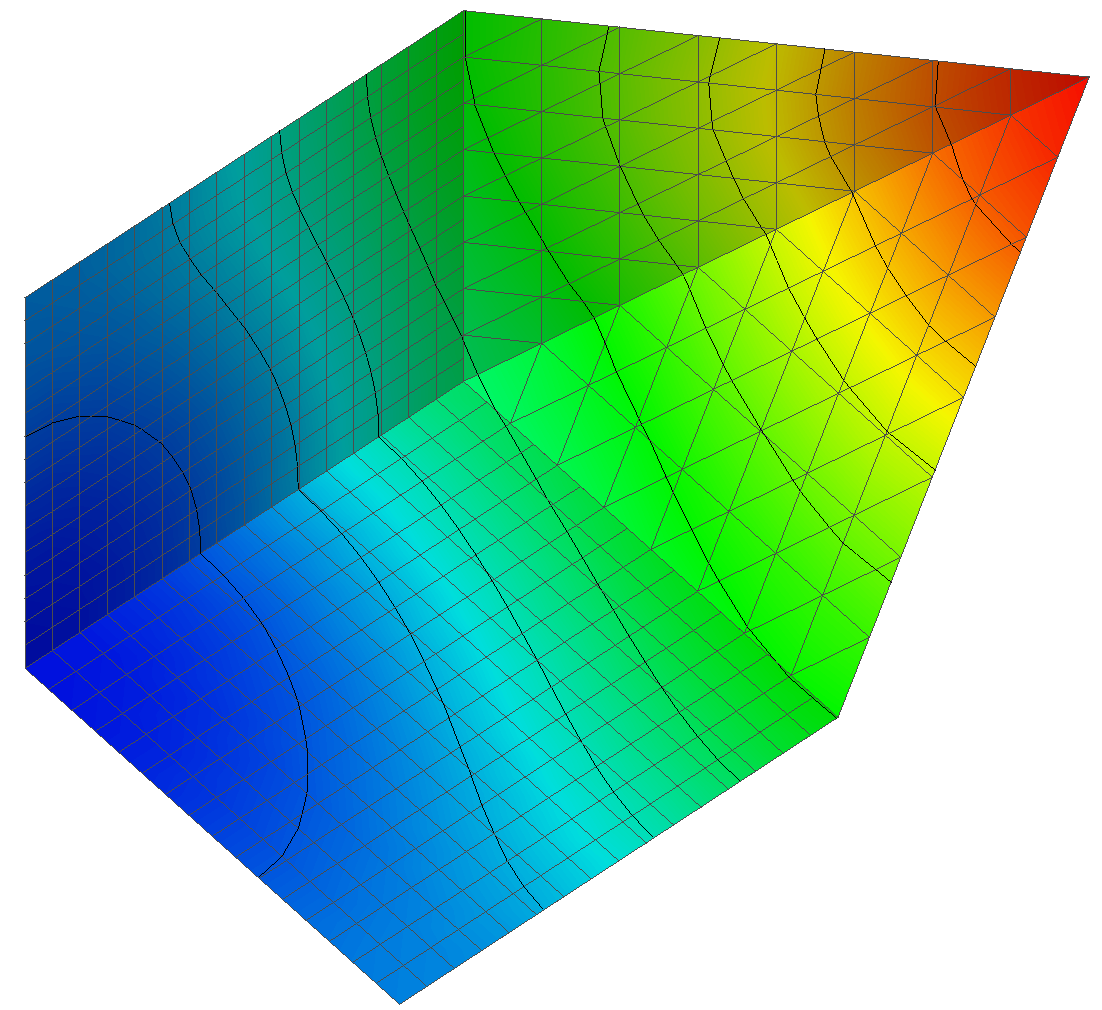
\includegraphics[width=.75\columnwidth]{figures/complicated_constrained}
    \caption{$h$-refinement for a simple Helmholtz problem using a
    hybrid prism/tetrahedral mesh.  Algebraic constraints enforce
    continuity across ``hanging nodes''\label{fig:amr_helmholtz}}
  \end{center}
\end{figure}
  

The error indicator work to date in \libMesh{} has focused on local
indicators that are essentially independent of the physics.  This
allows the library to be more flexibly applied in diverse applications.  On
the other hand, there is an extensive literature devoted to
obtaining more reliable \emph{a posteriori} estimates and accompanying
error indicators that are more closely linked to the operators and
governing equations for the application problem.  Bounds relating the
global error in energy to residuals with respect to the approximate
solution and governing equations have been developed and their
properties extensively studied.  Refinement indicators based on local
element residual contributions are a natural consequence and the most
common form of AMR indicator in the literature.  Recently, some more
precise and reliable indicators that involve the additional work of
solving a related dual problem have been proposed and are the subject
of ongoing
research~\cite{Bangerth2003,eriksson_1996,estep_2000,estep_2002,estep_2005}.
% I don't know this for sure...
%These dual indicators are being investigated using the toolkit
%\texttt{fetk}\footnote{\url{http://www.fetk.org}}
% Note: Michael Holst (UCSD) is a contributor to fetk, it is written in ANSI-C.
%% They can also be implemented in the open source library
%% \dealII{}\footnote{\url{http://www.dealii.org}}~\cite{Ban00i},
%% which influences the structure and direction of \libMesh{} as
%% discussed later.

Residual indicators and targeted dual
indicators are difficult to include in a flexible library without 
compromising the goal of physics-independence.  In the most general
case, an error estimator should be able to take only a finite element
mesh and a function expressed on that mesh and return approximate
error levels on every element.  \libMesh{} provides simple
interface derivative jump (or flux jump) indicators, the latter only
in the case where there is a discontinuity in material coefficient of
the flux vector across the element edge~\cite{kelly_error_1983}.
These only give rigorous error bounds for a very limited class of
problems, but, in practice, they have proved to be broadly applicable.
Another class of physics-independent indicators that is very widely
used because of their simplicity are the ``recovery indicators''.  In
this case the gradient or solution is recovered via local patch
post-processing~\cite{ZZ87}.  Superconvergence properties may be used
to provide a more accurate post-processed
result~\cite{wahlbin_superconvergence}.
A more rigorous foundation for these indicators has been
determined~\cite{varis_thesis}.
The difference between the more accurate
recovered local value and the previously-computed value provides the
local error indicator for the refinement process.  The ability for
error indicators to provide improved local solutions in addition to
error estimates is crucial for automatic $hp$ schemes, where in
addition to choosing which elements to refine it is also necessary to
choose how ($h$-subdivision or $p$-enrichment) to refine them.

There is a strong interest in utilizing parallel AMR/C in the setting
of the SIERRA framework being developed at Sandia National
Laboratory~\cite{sierra}.  Recovery indicators are being implemented
in SIERRA for many of the same reasons they are used in
\libMesh{}.  Sandia researchers are also engaged in collaborations
with University researchers to test and utilize the dual type
indicators.  To include such dual indicators in \libMesh{} for a
specific application we could add a residual calculation as a
post-processing step and then again utilize \libMesh{} for an
approximate solution of the linearized dual problem in terms of the
target quantity of interest using an ``appropriate'' mesh.  An
alternative model would be to solve the dual problem locally for an
approximation to this error indicator contribution.

The coarsening aspect of AMR/C merits further discussion.  Coarsening
occurs whenever a ``parent'' element is reactivated due to the
deactivation of all of its ``child'' elements.  This scheme assumes
the existence of an initially conforming mesh, whose elements
are never coarsened.  There are many practical issues related to the
selection of elements for refinement and coarsening, notwithstanding
the calculation of an accurate error indicator.
Special rules such as ``refine any element
which is already coarser than a neighbor chosen for refinement''
or ``refine any element which would otherwise become coarser than all
its neighbors'' may be chosen to smooth the mesh grading and
force additional refinement in regions with otherwise small error.

One of the approaches that we have been investigating is a
statistical strategy for proportioning cells between refinement and
coarsening.  The ideas are related to earlier
approaches~\cite{carey_gridbook} in which the mean $\mu$ and standard
deviation $\sigma$ of the indicator ``population'' are computed.
Then, based on refinement and coarsening fractions
$r_f$ and $c_f$ (either default values or specified by the user),
the elements are flagged for
refinement and coarsening.  This scheme, depicted graphically in
Figure~\ref{fig:ref_scheme}, is beneficial in
evolution problems where, at early times, the error is small and
equidistributed 
and no elements are flagged for refinement.  Later, as interesting
features develop, the statistical distribution spreads and
refinement and coarsening begins.  As the steady solution is
approached, the distribution of the error reaches a steady state as
well, effectively stopping the AMR/C process.
\begin{figure}[hbt]
  \begin{center}
    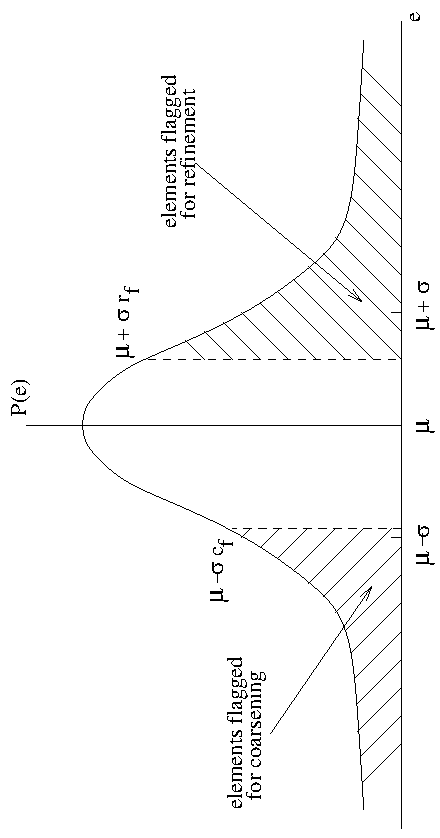
\includegraphics[angle=-90,width=\columnwidth]{figures/ref_scheme}
    \caption{In the statistical refinement scheme,
      the element error $e$ is assumed to have an approximately normal probability
      density function $P(e)$ with mean $\mu$ and standard deviation $\sigma$.
      Elements whose error is larger than $\mu + \sigma r_f$ are flagged for
      refinement while those with errors less than $e < \mu - \sigma c_f$ are flagged
      for coarsening.\label{fig:ref_scheme}}
  \end{center}
\end{figure}

We remark that other standard strategies for refinement and coarsening
are also used with \libMesh.
%% For example, the user may elect to refine
%% and coarsen fixed fractions of the elements at each step, or to refine
%% elements in which the error exceeds some percentage of the maximum
%% error in the mesh.
The optimal strategy for selecting elements for
refinement is somewhat problem-dependent and is an area of future
research.  Some further discussion is presented in
Section~\ref{sec:apps}.


%%%%%%%%%%%%%%%%%%%%%%%%%%%%%%%%%%%%%%%%%%%%%%%%%%%%%%%%%%%%%%%%%%%%%%%%%%%%%%
\section{Library Overview}
%\libMesh{} is certainly not the first software framework for adaptive
%finite element applications.
Experiences with a number of other
libraries demonstrated the feasibility of
developing high performance parallel numerical libraries in
\cpp{}~\cite{Ban00i,Alegra,scientific_engineering_cpp} and influenced
the \libMesh{} design.  As in \dealII{}, \libMesh{} was designed from
the beginning to use advanced features of the \cpp{} programming
language.  No provision is made for lower-level procedural languages
such as C or Fortran.  This is in contrast to other parallel
frameworks such as \Cactus{}\footnote{\url{http://www.cactuscode.org}}
or \ParFUM{}\footnote{\url{http://charm.cs.uiuc.edu/research/ParFUM}}.
However, exposing the class and template structure of \libMesh{} to
users can increase performance and facilitates extensibility, and both
are features we value above inter-language operability.
Some other high-performance library designs that have influenced
\libMesh{} are~\cite{ug_library,devloo_M2AN,demkowicz_hp}.

The \libMesh{} project began in March 2002 with the goal of providing
a parallel framework for adaptive finite element simulations on
general unstructured meshes.  The library is distributed under an
open-source software license and hosted by
\Sourceforge{}. Geographically dispersed development is ma\-naged with
the Concurrent Versions System (\CVS) software.  The online
documentation for the library has averaged approximately 40,000 hits a
month since January 2005.  The library itself has been downloaded on
average approximately 150 times a month.

\subsection{Scope}
The library was originally intended to provide a powerful
data structure which supports adaptive mesh refinement for
arbitrary unstructured meshes arising in finite element and finite
volume simulations.  By separating the adaptive meshing technology
from the application code, the potential for code reuse increases
dramatically, and this is evident from the growing number of diverse
applications which now exploit the library.  Some application
results are presented in Section~\ref{sec:apps}.

Subsequent development efforts have been targeted at increasing
performance, supporting more general classes of finite elements, and
implementing specific solution algorithms for transient and nonlinear
problems.  A major goal of the library is to provide support for
adaptive mesh refinement computations in parallel while allowing a
research scientist to focus on the physics being modeled.  To this
end the library attempts to hide complications introduced by parallel
computing whenever possible so that the user can focus on the
specifics of the application.

Both AMR and parallelism offer means to accelerate simulation and
analysis for design and rapid prototyping: parallel speed-up reduces
the real time to solution and likewise AMR permits a solution to be
achieved to comparable accuracy on a coarser but better designed mesh
than with standard non-adaptive meshing.
%% To illustrate the effects
%% of these approaches one could envisage a pie-chart depiction of the
%% class of all applications that can be solved.  Then, because of memory
%% and solution time constraints, only a small wedge of the pie chart
%% would correspond to those problems that could be solved on a typical
%% workstation by an engineer or scientist using standard meshes and
%% serial computation.  Next, let us make the reasonable assumption that
%% on average adaptive meshing is able to solve the problem with similar
%% reliability using an order of magnitude fewer node points.  There is a
%% corresponding reduction in memory requirements and even greater
%% speedup in solve time.  Alternatively, one could solve a more
%% complicated problem with a comparable number of mesh points that are
%% now well distributed by AMR and in the same time as the previous
%% standard mesh simulation.  This implies a much larger wedge of the pie
%% chart corresponds to the application class that can now be addressed
%% when the new AMR capability is added.If instead of introducing AMR one
%% implements distributed parallel solution of the problem on, say, a
%% workstation cluster, then again a much larger problem could be solved
%% in the same real time because the parallel cluster is able to divide
%% the work and memory requirements across the processors.  Hence again,
%% a larger wedge of the pie would define the new range of applicability
%% of analysis due to parallelism.  In both instances( AMR and
%% parallelism), there are still resource limitations that determine how
%% large a problem can be admitted with either adaptivity or with
%% parallelism.For example, some common information may reside on all
%% processors and AMR has additional overhead associated with the
%% refinement ``tree.''
The goal in combining adaptivity and parallelism is clearly to reap
the benefits of both techniques in being able to solve problems more
efficiently and in shorter real time or, alternatively, being able to
consider more complicated problems with a fixed set of resources.  Of
course, when one utilizes AMR or parallelism, additional layers of
complexity are being added to the analysis problem, methodology,
algorithms, data structures and software.  There is also an overhead
associated with the implementation of both AMR and parallelism and
these factors should also be taken into account.  Nevertheless, it is
clear that each of these strategies offers the ability to greatly
enhance the computational capability available to a researcher.

\subsection{\cpp{} and Scientific Computing}
The library is written in \cpp, with code designed for the ISO
standard but tested and restricted for compatibility with older Intel,
IBM, GNU, and other compilers.  The library uses polymorphism to
enable a separation between application physics and finite element
implementation.  The support for object-oriented programming in \cpp{}
allows application authors to write their code around abstract class
interfaces like \texttt{FEBase}, \texttt{QBase}, and
\texttt{NumericVector}, then to switch at compile time or run time
between different finite element types, quadrature rules, and linear
solver packages which implement those interfaces.  To reduce the
overhead of virtual function calls to abstract base classes, we
provide methods which encourage developers to use a few calls to large
functions rather than many calls to small functions.  For example,
sparse matrices are constructed with one function call per element to
add that element's cell matrix, rather than directly calling virtual
\texttt{SparseMatrix} access functions for each degree of freedom pair
at each
quadrature point.  For frequently called functions which cannot be
combined in this way, \libMesh{} uses \cpp{} templates.  We mimic the
support for generic programming in the \cpp{} Standard Template
Library.  For example, \libMesh{} iterator classes make it easy for
users to traverse important subsets of the elements and nodes
contained in a mesh.

Our decision to use \cpp{} is much in the spirit of Winston
Churchill's famous opinion of democracy: ``It is the worst system,
except for all the others.''  This philosophy, advanced by the
\texttt{Alegra}~\cite{Alegra} developers in the mid 1990s, is still
germane today.  Although writing efficient \cpp{} code can be
difficult, the \cpp{} language supports many programming styles, making it
possible to write software with layers of complexity which are more
easily maintainable than in
``lower level'' languages (e.g.\ C, Fortran)
but with time-critical routines that have been
more aggressively optimized than is possible in ``higher level''
languages.  Fortran and C are fast and popular languages for numerical
analysis, but do not adequately support the object-oriented
methodology we wanted for \libMesh.  Java implements run time
polymorphism via inheritance, but lacks the compile time polymorphism
that \cpp{} templates provide to produce faster executables. Java also
lacks the operator overloading that \libMesh{} numeric classes like
\texttt{Vector\-Value} and \texttt{Tensor\-Value} use to make formulas
look more natural to a mathematician.

The existence of high-quality standards-conforming \cpp{} compilers
from hardware vendors, software vendors, and the GNU project helps
keep \libMesh{} portable to many different hardware platforms.  The
ease of linking C, Fortran, and assembly code into a \cpp{}
application also allows \libMesh{} to make use of existing libraries
written in lower-level languages.  Also, \cpp{} encapsulation provides
a natural mechanism for interfacing with separate third-party
libraries through a common interface (as discussed in
Section~\ref{sec:libraries}), and object-oriented design is
well-suited for handling the layers of complexity introduced by
combined adaptivity and parallelism. \ICESOnly{There is a rich
selection of third party development tools available for \cpp{} as
well.  Profiling and performance monitoring classes are built into
\libMesh{}, for example, but fine grained performance optimization is
still most easily done with third party compiler and profiler
support.}  Finally, \cpp{} ranks with C and Java as one of the most
popular programming languages among software developers, which has
helped attract more end users to the \libMesh{} library and more
external contributors to \libMesh{} development.


\subsection{Open Source Software Development}
The library and source code are distributed under the GNU Lesser
General Public License (LGPL)~\cite{gnu_lgpl}.  The LGPL provides the
benefits of an open source license but also allows the library to be
used by closed source and commercial software.  This is important for
the research community, because it allows applications using the
library to be redistributed regardless of the application's license.
In January 2003, the popular \Sourceforge{} site was chosen to host
the first official software release.  \Sourceforge{} provides
services to aid software development including \CVS{} repository
management, web\footnote{\url{http://libmesh.sourceforge.net}} and
database hosting, mailing lists, and access to development platforms.

The \CVS{} branch hosted at \Sourceforge{} is frequently updated by the core
group of authorized developers.  Periodically the developmental branch
is ``frozen'' in order to create an official release.  During each
freeze, major API changes are deferred while outstanding problems in
the code are fixed and the library is tested on each supported
platform to ensure portability.
The public has \CVS{} read access, so users can periodically modify
their application codes to take advantage of new library features, or
simply tie their application to a particular \libMesh{} version.

Developers are sometimes recruited from the user community,
when a user desires a specific library feature and,
with help from the other developers, submits the new functionality
as a patch to the current \CVS{} tree.  After testing the patch, an
authorized developer can check it in to the active branch.
Users who want to make significant, continuous
improvements to the library are added as active
developers and given \CVS{} write access.

Accurate documentation is critical for the success of any \cpp{} class
library.  In \libMesh{} the well-known \texttt{doxygen} utility is
used to extract documentation directly from source
code~\cite{using_doxygen}.  This approach has the benefit of keeping
the source code and its documentation synchronized.  \texttt{doxygen} extracts
blocks of comments and creates a well-organized web page which
contains class documentation, detailed inheritance diagrams, and
annotated source code.


\subsection{Interfaces to Other Libraries\label{sec:libraries}}
There are a number of existing, high-quality software libraries that
address some of the needs of a simulation framework.  In \libMesh, we
utilize existing software libraries whenever possible. It is
crucial for a small development team to avoid the ``not
invented here'' mindset, so that efforts may be focused as narrowly
and effectively as possible.  The most general support for third party
software such as the hex mesh generator CUBIT~\cite{CUBIT} is provided
through the mesh file format support discussed in
Section~\ref{sec:mesh}, but \libMesh{} can also be configured to
directly link to supporting software when convenient.  Some third
party libraries in addition to the ones discussed below include the
\boost{} \cpp{} source libraries, the 2D
Delaunay triangulator \Triangle{}~\cite{shewchuk96b}, and the 3D
tetrahedral mesh generator \tetgen~\cite{tetgen_manual}.

The library uses both METIS~\cite{karypis:metis} and
ParMETIS~\cite{karypis:parmetis} for domain decomposition (discussed
further in Section~\ref{sec:dd}).  The Zoltan library from Sandia
National Labs provides a uniform interface to a number of mesh
partitioning schemes~\cite{ZoltanOverviewArticle} and would be natural
to include in the future.  Additional partitioning schemes can be
added to the library very easily through the standard \cpp{} approach
of subclassing.  The library provides the abstract \texttt{Partitioner}
base class that defines the partitioning interface, and derived classes
can serve as wrappers for external partitioning libraries.

The base class/derived class paradigm is also used to interface with
third party linear algebra packages.  In this case the library provides
the abstract \texttt{Sparse\-Matrix}, \texttt{Numer\-ic\-Vector}, 
\texttt{Linear\-Solver}, and \texttt{Eigen\-Solver} classes.  Derived
classes are then used
to provide the actual implementation.  This approach has been used to
encapsulate the interface to solver packages such as
LASPack~\cite{laspack_manual}, which provides Krylov subspace linear
solvers for serial machines, \PETSc{}, the parallel
scientific computing toolkit from Argonne National
Labs~\cite{petsc-efficient}, and \SLEPc{}, the library for
eigenvalue problem computations from Universidad Politecnica de
Valencia~\cite{slepc_acm}.

\subsection{Portability}
Portability across a number of platforms using native compilers has
been a goal of the library design since its inception.  The bulk of the
development work is performed on Linux desktop machines using the
\href{http://gcc.gnu.org}{GNU Compiler Collection}, but a number of
other platforms are supported as well.  The library makes extensive
use of the \cpp{} Standard Template Library, so it is essential to use
multiple compilers to ensure compiler-specific constructs are avoided.
\ICESOnly{
Because \libMesh{} is an open source application, compatibility with
even old and non-standards-compliant compilers is an important way to
make the library accessible to new developers.  Functionality which is
now part of the \cpp{} standard but which was not immediately
supported by popular compilers is still used in \libMesh{} via
compatibility classes like \texttt{AutoPtr} and
\texttt{OStringStream}, which reimplement the standard interfaces in
ways pre-standard compilers can understand.
}

The GNU \autoconf{} package is used to configure the library for
a given installation.  This approach uses the familiar
\texttt{configure} script to probe a user's computing environment for
parameters such as compiler and external library versions.
The configuration process also
sets global options such as whether real or
complex-valued scalars are to be used.  This procedure produces a
custom \texttt{Makefile} with site-specific
information, and the library is built with GNU \make{} or the
vendor equivalent.

The desire to use native compilers is primarily performance driven.
On architectures such as the IBM Power~5 and the Intel
Itanium\small$^{\textregistered}\!\!$\normalsize~II there are a number of
complex instructions available, and vendor-supplied compilers seem to
optimize well for these features.  Additionally, when a new platform
becomes available it is often vendor-supplied compilers which are
available first.  For these reasons the library has always been tested
with a range of compilers before each official release.  A side effect
of this approach is that the library has subsequently been ported to
additional architectures such as OSX and Windows with little
difficulty.

One ongoing issue is portability across different versions of external
libraries such as \PETSc.  The \PETSc{} API often changes between
minor releases, rendering code that was correct for one version
inoperable with another.  GNU \autoconf{} and the C preprocessor are
used to provide the correct code for the installed version of
\PETSc{}, and modifications are inevitably required with each
subsequent \PETSc{} release.  At the time of this writing, \libMesh{}
supports all versions of \PETSc{} from 2.1.0 to 2.3.0.
One way of getting around such issues is to actually distribute
the source code for external libraries with \libMesh.  This approach
is used for LASPack and \tetgen, but is impractical for PETSc due to
its size and build complexities.


%%%%%%%%%%%%%%%%%%%%%%%%%%%%%%%%%%%%%%%%%%%%%%%%%%%%%%%%%%%%%%%%%%%%%%%%%%%%%%
\section{Domain Decomposition\label{sec:dd}}
A standard non-overlapping domain decomposition approach is used in
\libMesh{} to achieve data distribution on parallel computers as shown
in Figure~\ref{fig:orbiter_dd}~\cite{carey_gridbook}.  The discrete
domain $\Omega_h$ is partitioned into a collection of subdomains:
$\left\{\Omega_h^p\right\}$ such that $\bigcup\Omega_h^p=\Omega_h$ and
$\bigcap\Omega_h^p=\emptyset$. The elements in each subdomain are
assigned to an individual processor.
\begin{figure}
  \begin{center}
    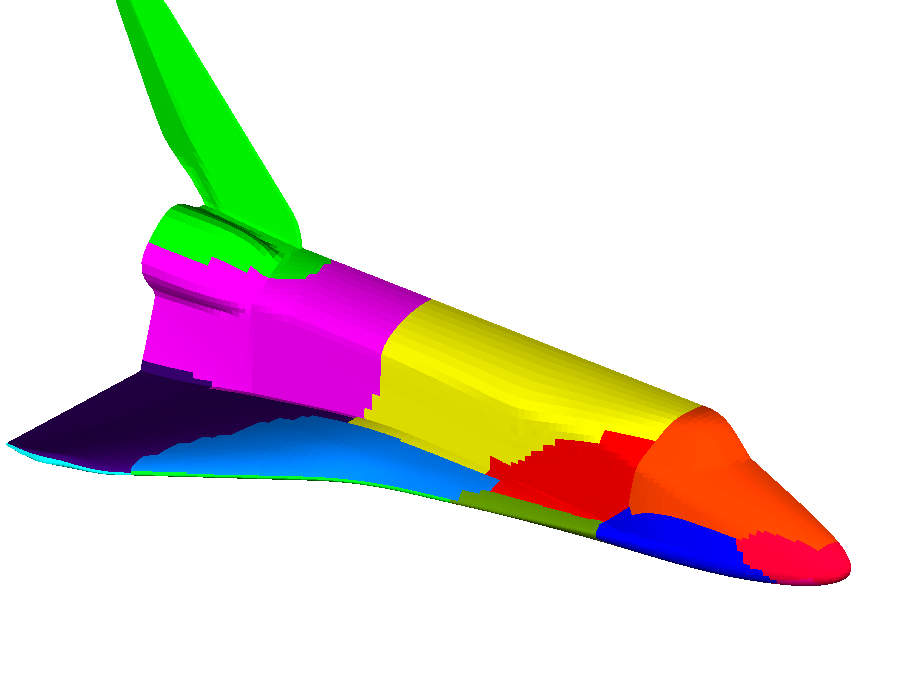
\includegraphics[width=\columnwidth]{figures/orbiter_surface}
    \caption{Element-based domain decomposition of a surface mesh
      into 16 subdomains\label{fig:orbiter_dd}}
  \end{center}
\end{figure}
The two primary metrics in judging the quality of a partition are the
subdomain mesh size and the number of ``edge cuts'' in the resulting
partition.  For a mesh composed of a single type of element,
each subdomain should contain an equal number of elements so that the
resulting domain
decomposition is load balanced across all available processors.  The
edge cut metric, on the other hand, is designed to minimize the
interprocessor communication required by the parallel solver.
For an overview of several domain decomposition strategies
which are available, see~\cite{iqbal_carey_2005,ZoltanOverviewArticle}.

In problems with high-resolution static meshes, the partitioning is
only performed once.  In such cases, a high-quality 
partition which simultaneously minimizes both the
size and edge-cut metrics may be desirable even though it is
relatively expensive.  For AMR/C
applications where the steady-state solution is of interest, it is
frequently the case that one begins with a coarse mesh at the root
level and progressively refines towards a near-optimal mesh with
little coarsening. It is obvious that an initially balanced partition
may rapidly become very unbalanced here and lead to computational
inefficiencies. Consequently, the mesh typically requires frequent
repartitioning during the AMR process. The development of optimal
schemes for
repartitioning that can take advantage of a prior partition in a
parallel AMR setting is still an open research
issue~\cite{iqbal_carey_2005}.

In \libMesh{} we partition by default with the recursive scheme
provided by METIS when the number of selected partitions $n_p \leq8$,
and with the k-way scheme otherwise.  A space filling curve
partitioning algorithm is also available, as is an interface to
ParMETIS.  The frequency of repartitioning needed will in general
depend on the evolving imbalance, and can occur as often as every time
the mesh changes (i.e. every time refinement or coarsening occurs).
Profiling suggests that this technique is not overly inefficient for
typical applications, but it could be very slow for large-scale
problems, and clearly it is unnecessary if the refinement scheme
selects only a small number of elements to be refined and
coarsened. This is one of many aspects of algorithmic performance
which must be considered for a given application on a given computer
platform.  For further discussion see Section~\ref{sec:apps}.

Another issue that must be considered is the subset of the AMR tree on
which the partitioning algorithm acts. Typically, the partitioning
algorithm is applied to all the active elements (i.e., the leaves of
the AMR tree) so that subsequent calls to the matrix assembly routine
can be effectively parallelized.  However, this may involve calling
the partitioning algorithm on a large subset of the AMR tree when it may
be sufficient to partition based on a coarser level and simply assign
all the children of these coarse level elements to the same processor.
Due to the parallel implementation of the \texttt{Mesh} discussed in
Section~\ref{sec:parallel_issues}, we do not (yet) consider the
possibility that accessing an ancestor element would require
off-processor communication.  In such a scenario, one would need to
ensure that repeated refinement and coarsening of the same element
did not lead to excessive communication overhead, perhaps by ensuring
that a local synchronized copy of an element's parent is always available.




%%%%%%%%%%%%%%%%%%%%%%%%%%%%%%%%%%%%%%%%%%%%%%%%%%%%%%%%%%%%%%%%%%%%%%%%%%%%%%
\section{Data Structures}
This section describes several of the key data structures in
\libMesh{}.  The discussion focuses on basic functionality, possible
extensions, and the reasoning behind certain design decisions.  
Algorithms that are central to the library's functionality are also
described.

\subsection{Mesh\label{sec:mesh}}
The \texttt{Mesh} class is central to \libMesh{} and was one of
the first developed.  It provides a discrete description of an
object in $d$-dimensional space, where $d$ is 1, 2, or 3.  The
discretization is composed of elements and nodes which are stored in
the mesh, but the manner in which these data are stored is encapsulated
by abstract classes with implementation-indepen\-dent
interfaces.  This data encapsulation has allowed for
re-factoring of the mesh class with minimal impact on the external
application programming interface.

A base class/derived class structure is used to implement mesh I/O in
various formats.  Virtual base classes describe the interface for mesh
input and output, and derived classes provide the actual I/O
functionality.  The library supports reading and writing a
number of unstructured mesh formats, including the UCD format from
AVS, the I-deas Universal format UNV, Exodus~II from Sandia National
Labs, GMSH, TetGen, Tecplot (ASCII and binary) and GMV from Los
Alamos National Labs.  The initial mesh is assumed to be conforming
and provides the level-0 parent elements in the refinement hierarchy
described in section~\ref{sec:elements_hierarchy}.

Custom iterator objects can be created to provide access to the
elements and nodes contained in a mesh.  The user can instantiate
iterators to access all the elements in the mesh or some meaningful
subset thereof.  The latter approach is useful, for example, during
parallel finite element matrix assembly on an adaptively refined mesh.
In this case, the user obtains iterators which traverse the set of
active elements (described in more detail in
section~\ref{sec:elements_hierarchy}) which are owned by the local
processor.

The mesh class is designed to be extensible.  Encapsulating
the stored elements and nodes by providing access only through
custom iterators admits the possibility of providing different
implementations for specific instances.  The \texttt{Mesh}
implementation assumes a fully unstructured, hybrid element mesh. 
However,
algorithmic and storage-based optimizations for Cartesian grids,
block-structured grids, and grids with only a single type of element
could be added without changing the current interface.


\subsection{Degrees of Freedom\label{sec:dof_distribution}}
The first finite elements implemented in \libMesh{} were the standard
Lagrange elements with nodal value degrees of freedom.  The library
has since been extended to a wider variety of finite element types
(see section~\ref{sec:element_spaces}).  Shape functions on more
exotic finite elements can correspond to nodal Hessian components,
mid-edge normal fluxes, or orthogonal hierarchic polynomials.
%% Clearly, the ``degree of freedom'' concept must extend beyond
%% the simple one-to-one nodal correspondence of Lagrange elements.
For these finite element types, it no longer makes sense to associate
each shape function with a single geometric point.

The \texttt{DofObject} class handles these different types of 
degrees of freedom generically.  Examples of \texttt{DofObject}s
are element interiors, faces, edges, and vertices.  An element interior
has associated degrees of freedom for those shape functions whose
support is contained within the element.  Face degrees of
freedom correspond to shape functions contained within the two
elements sharing a face, edge degrees of freedom correspond to shape
functions for all elements sharing an edge, and vertex degrees of
freedom correspond to shape functions supported on all elements
sharing a single vertex.
%% Admitting multiple degrees of freedom per node, for
%% example, allows this data structure to handle any finite element space
%% with a locally supported basis.  (A discussion of the finite element
%% spaces currently supported in the library is presented in
%% section~\ref{sec:element_spaces}.)

The domain decomposition approach described earlier assigns disjoint
groups of elements to individual processors.  This allows the
element-based degrees of freedom to be assigned uniquely to the
processor which owns the element, but requires some shared
distribution of vertex, edge, and face degrees of freedom.
Figure~\ref{fig:dofs_dd} illustrates the approach which is used in the
library. In this approach, any degrees of freedom on the border
between subdomains are owned by the processor of lowest
global index.  This is evident from the figure, where the nodes on the
shared interface have been assigned to processor~0.
\begin{figure}[hbtp]
  \begin{center}
    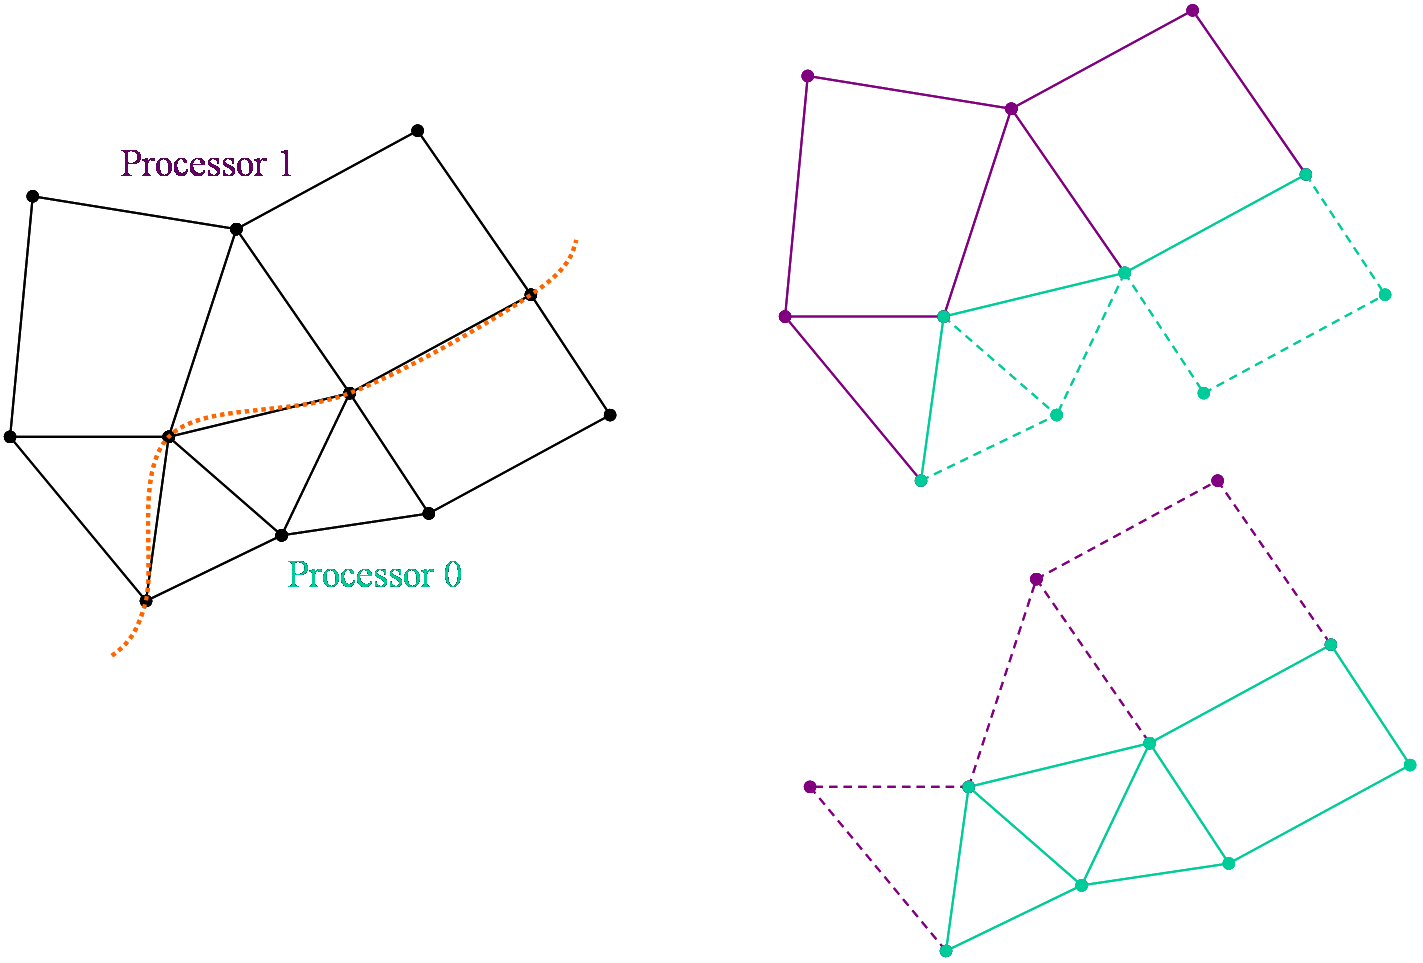
\includegraphics[width=\columnwidth]{figures/dofs}
    \caption{Element partitioning \& degree of freedom
      distribution.  Disjoint element sets are divided between
processors, while boundary nodes are assigned to the processor with
lower ID.\label{fig:dofs_dd}}
  \end{center}
\end{figure}

This approach for assigning degrees of freedom to processors also fits
well with the sparse matrix partitioning scheme employed in \PETSc{},
where complete rows of the sparse matrix are assigned to individual
processors~\cite{petsc_manual}.  This is the natural matrix
decomposition that results from the degree of freedom distribution
used in the library.

\subsection{Nodes}
Each object of the \texttt{Node} class stores its $(x,y,z)$ location
in space, as
well as additional state information including a unique global identification
number (ID) and degree of freedom indices.  The mesh data structure
contains a complete list of all nodes.  Nodes may be accessed directly
by the user via iterators, or indirectly through elements which are
connected to the nodes. Trivial operations such as scaling,
translating, or rotating a mesh are performed directly on the nodes.

During the refinement process new nodes may be added to the mesh.
When two adjacent elements are refined, common nodes will exist on the
inter-element interface. This situation must be properly resolved to
achieve a valid discretization (i.e. with no duplicate nodes).  A new
node is
created as a linear combination of existing nodes, and a hash key is
constructed for each new node based on the weights and global IDs of
its parent nodes.  If this key already exists in the map of new node
keys, the new node is a duplicate and is therefore rejected.  This
procedure efficiently resolves nodal connectivity for refined
elements.

Similarly, coarsening the mesh can create ``orphan nodes,'' or nodes
that are not connected to any elements.
%In our initial implementation
%these orphan nodes were retained, so that they could be 
%re-connected to future elements that may appear in the refinement
%process.  For example, in transient applications with
%some periodic behavior, elements will be created and destroyed
%repeatedly, and avoiding node deallocations and reallocations could
%speed up element
%refinements.  However, numerical experiments indicated that this approach did
%not provide an appreciable speedup, and the default behavior is now to
%remove orphan nodes.
After an AMR/C step the library simply counts
the number of elements connected to each node and removes those nodes
which are not connected to any elements.


\subsection{Elements}
\libMesh{} defines the abstract base class \texttt{Elem} which
defines the interface for a geometric element.  Concrete
subclasses of \texttt{Elem}, such as \texttt{Quad4} and
\texttt{Tet10}, are specialized via virtual function calls to return
e.g. the correct number of nodes and sides when \texttt{n\_nodes()} and
\texttt{n\_sides()} are called on an \texttt{Elem} pointer.  The
complete list of geometric element types provided in \libMesh{} is shown in
Figure~\ref{fig:elem_class}.
\begin{figure}
  \begin{center}
    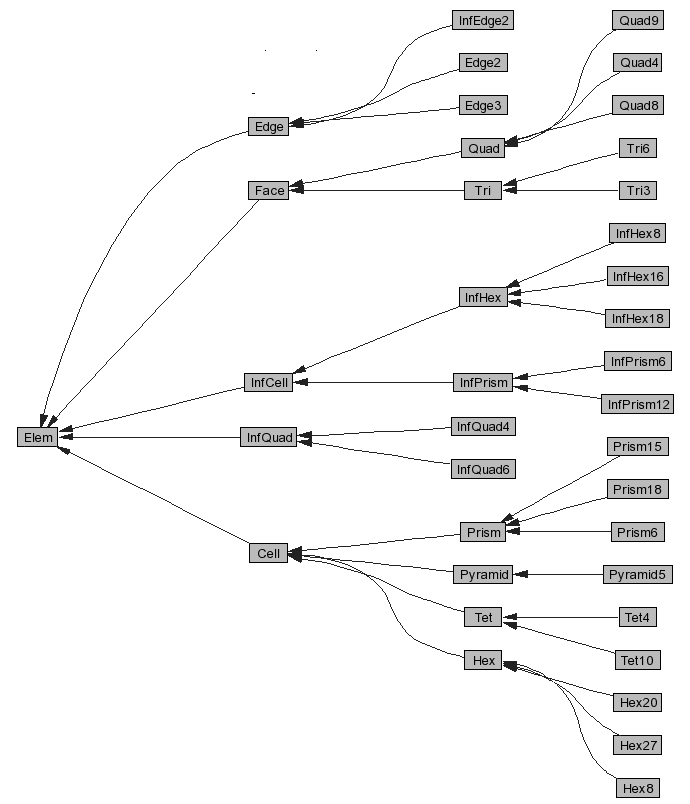
\includegraphics[width=\columnwidth]{figures/inherit_graph}    
    \caption{The \texttt{Elem} class hierarchy\label{fig:elem_class}}
  \end{center}
\end{figure}
Note that an \texttt{Edge} \emph{is} an \texttt{Elem} (in the polymorphic
sense) in 1D, and similarly for \texttt{Face} in 2D and \texttt{Cell} in 3D.
Implementations of all the standard geometric element types used in finite
element analysis including quadrilaterals, triangles, hexahedra, tetrahedra,
prisms, and pyramids, as well as a collection of infinite elements, are
provided in \libMesh.

\subsubsection{Nodal Connectivity\label{sec:elements_connectivity}}
Elements contain state information similar to nodes.  Elements store a
unique ID, their processor ID, and degree of freedom information.
Additionally, the element connectivity is stored as pointers to nodes.
This is a slight departure from the classic finite element data
structure, in which the element connectivity is defined in terms of
the nodal indices~\cite{becker_carey_oden_volume_1}.  On 32-bit
machines pointers and integers are both 4~bytes, so this choice does
not impose additional storage.  On 64-bit machines, however, pointers
are 8~bytes, which essentially doubles the amount of memory required
to store element connectivity.

This approach for storing the element connectivity was chosen so that
elements could have increased functionality in the absence of a
corresponding \texttt{Mesh} object.  A traditional connectivity scheme
would require the mesh to access the nodal locations of a given
element.  This is important, for example, when computing the map from
a physical to reference element or determining if a point lies inside
an element.  By storing pointers to the nodes, the element can
determine its geometric connectivity directly.  This simplifies many
functions in the code by requiring the user to pass only an element
instead of both an element and the nodal locations.  Additionally,
this approach reduces the amount of indirect memory addressing
required for an element to obtain nodal information.

\subsubsection{Face Neighbors\label{sec:elements_neighbors}}
Elements also store pointers to their face neighbors.  Two elements
are said to be face neighbors if they share a ``side,'' where a
``side'' is a \texttt{Node} in 1D, an \texttt{Edge} in 2D, and a
\texttt{Face} in 3D.  If an element side is on the physical boundary
of the domain there will be no neighbor.
%% This is indicated in the code by a \texttt{NULL}
%% pointer, hence locating the elements coincident with the boundary is
%% equivalent to finding all the elements with a \texttt{NULL} neighbor.
Locating the elements coincident with the boundary is equivalent
to finding all the elements which have at least one side with no
neighbor. This is useful when applying boundary conditions.

After reading a mesh from disk, or performing mesh refinement, it is
necessary to construct the face neighbor information efficiently.  The
library handles this by looping over all the elements and then over
the sides of the elements.  If a neighboring element has not been
located already the side of the element is constructed and a hash key
is computed based on the global indices of its nodes.  A map is then
queried to find any elements with sides matching this key, and they
are checked for a possible match.  The loop through the $N$ elements
is $O(N)$, while for a map of size $M$ the lookup is $O(\log M)$, so
the resulting algorithm has $O(N\log M)$ complexity. With 
$M \le N$, this yields a potentially $O(N\log N)$
algorithm.  Alternate approaches are possible for which $M \ll N$
which could improve performance for very large meshes.  For example,
ordering the elements with a space-filling curve before performing the
neighbor search will ensure adjacent elements are quickly located,
reducing the overall size of the map.

Since constructing the side of an element is a common task, a special
proxy class called \texttt{Side} has been developed for this purpose.
This class essentially defines the side of an element as a new element
living in a lower spatial dimension and provides the connectivity
through a mapping from the original element.  This approach allows the
side of an element to be constructed rapidly, as the allocation and
population of a new connectivity array is not required.

\subsubsection{Element Refinement Hierarchy\label{sec:elements_hierarchy}}
Elements are refined upon user request via the ``natural refinement''
scheme.  In this approach $d$-dimensional elements are generally
refined into $2^d$ subelements of the same type. (Pyramid refinement
is an exception to this rule: refining a pyramid results in a
collection of pyramids and tetrahedral elements.)  Hanging nodes are
allowed at element interfaces and hanging degrees of freedom are
constrained algebraically. This approach was chosen because it is
applicable for general hybrid meshes with arbitrary types of elements,
and in general results in refined elements of the same type.  This
latter point ensures that refining an all-quad mesh in 2D produces an
all-quad mesh, for example.
\begin{figure}
  \begin{center}
    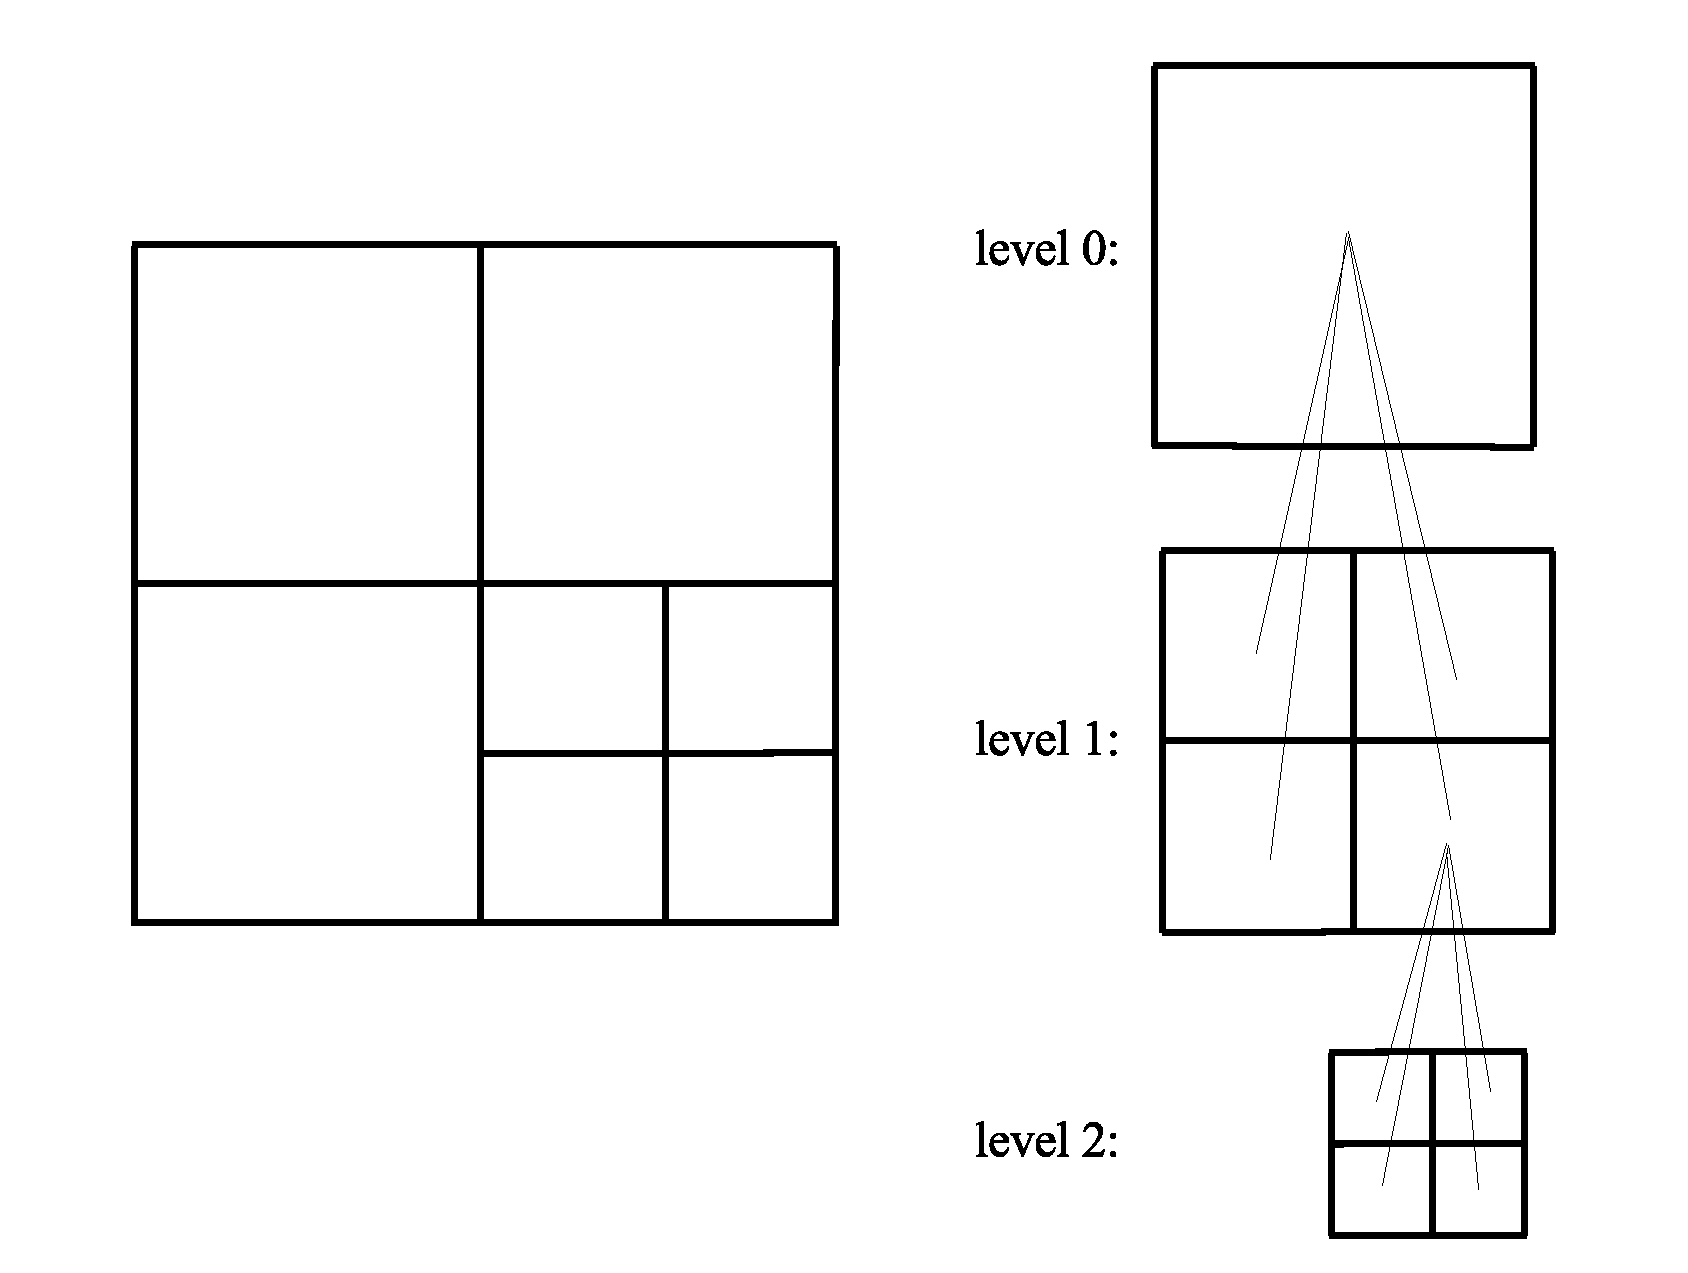
\includegraphics[width=\columnwidth]{figures/hierarchy}
    \caption{Element refinement hierarchy and resulting quadtree for a 2D quadrilateral mesh.\label{fig:hierarchy}}
  \end{center}
\end{figure}

This refinement approach naturally yields a tree data structure, and
Figure~\ref{fig:hierarchy} shows the quad tree data structure which
results from refining a single quadrilateral element.  Each element
has a pointer to its ``parent,'' and an array of pointers to its
``children.''  The initial, level-0 elements are unique in that they
have no parent.  Similarly, the active elements which are used in
finite element computations have no children.  The level of a given
element is determined recursively from its parent.  The user is
allowed to access any subset of the elements via iterators as
discussed previously.  The active elements are commonly used in matrix
assembly, but intermediate levels could also be used in a multigrid
cycle, for example.

The element hierarchy is additionally used to locate hanging nodes in
the mesh which must be constrained.  As mentioned previously, elements
store pointers to neighboring elements which share sides.  These
neighboring elements are necessarily at the same level of refinement.
If an active element's neighbor is a refined element, then any degrees
of freedom located on the common side must be constrained.

The refinement hierarchy also naturally supports element
coarsening. In the case that all of the children of an element are
flagged for coarsening, the parent element simply deletes its
children and becomes active again.
In Figure~\ref{fig:hierarchy}, this would correspond to all the
level-2 elements being deleted.  The resulting mesh would contain just
the active level-1 elements and their parent.  A consequence of this
approach to element coarsening is that the mesh cannot be coarsened
below the initial, level-0 mesh.  In many cases it is desirable to
use the coarsest level-0 mesh possible and allow the refinement
process to add elements only where they are needed.

\subsection{Systems}
The abstract \texttt{System} class in \libMesh{} corresponds to a PDE
system of one or more equations that is to be solved on a given mesh.
\libMesh{} provides several concrete system implementations including
explicit, implicit, steady, transient, linear, and nonlinear systems.
A system stores the solution values for the degrees of freedom in a
simulation, which may be either real- or complex-valued.  Additionally,
a system may contain additional information such as a sparse matrix,
which is required for implicit solution strategies.  In the current
implementation a system is uniquely tied to a given mesh, so a
simulation that uses multiple meshes must also solve multiple systems.

The \texttt{System} class provides a generic, customizable interface
which allows the user to specify the physics-dependent parts of an
application.  For example, in the case of an implicit system users can
provide a function for matrix assembly or can derive their own class
and overload the matrix assembly operator.  Similarly, for transient
systems the user may either provide an initialization function or
overload the initialization operator provided in the library.

\ICESOnly{
Subclasses of \texttt{System} are included in \libMesh, to provide
additional support for common problem types through supersets of the
base interface.  The \texttt{ExplicitSystem},
\texttt{LinearImplicitSystem}, \texttt{NonlinearImplicitSystem},
\texttt{EigenSystem}, \texttt{FrequencySystem}, and
\texttt{NewmarkSystem} each provide the extra data structures and code
required for their particular variety of PDE.
}

Multiple systems may be tied to a given mesh to allow for loose
coupling of different physics.  This feature has been applied in the
case of Rayleigh B$\acute{\text{e}}$nard Marangoni flows to decouple
the incompressible fluid flow and heat transfer equations.  In this
example two implicit systems are solved in an iterative fashion.
Similarly, incompressible flows using pressure projection
operator-splitting techniques have been solved using a combination of explicit
and implicit systems.

The library makes extensive use of \cpp{} templates to allow
complicated systems to be constructed from simpler subsystems.  For
example, transient nonlinear systems are supported by combining a
transient outer loop with a nonlinear inner loop.  Templates are
useful in this setting because they allow simple components to be
combined into a complex algorithm. This enhances code reuse and
minimizes debugging efforts.
%FIXME: add an example of code (at least for ICES report) here?

\subsection{Finite Element Spaces\label{sec:element_spaces}}
The library provides a number of finite element ``families'' that may
be used in a simulation.  The classic first and second order Lagrange
finite elements are supported, as well as $C^0$ hierarchic elements
of arbitrary polynomial order.  Mapping between physical and
computational space is performed with the Lagrange basis functions
that are natural for a given element.  For example, mapping of a
three-node triangle is performed with the linear Lagrange basis
functions, while a 27-node hexahedral element is mapped with a
tri-quadratic Lagrange basis.  For many mesh geometries, quadratic Lagrange
elements are only mapped linearly from computational space.
Provisions are made in the library to detect this and use the minimal
polynomial degree required for an accurate map.

Discontinuous finite element spaces are also supported.  For these
approximation spaces the degrees of freedom are wholly owned by the
elements.  The library offers monomial finite element bases for these
spaces.  One approach is to use the monomial basis defined in terms of
the reference element $(\xi,\eta,\zeta)$ coordinates for each element
in the domain.  Another option is to use the physical $(x,y,z)$
coordinates inside the element as the monomial basis.  The former
approach is efficient when the discontinuous spaces will be used
primarily for integration inside the element (such as the LBB-stable
$Q_2P_{-1}$ quadrilateral element for incompressible
flows~\cite{Gres-1998}), while the latter approach is attractive for
the many element boundary computations which arise in the
discontinuous Gale\-r\-kin family of finite element methods and in
finite volume discretizations.

% FIXME: figures for different element spaces in ICES report?

Support for $C^1$ continuous elements is provided in the library.
Users can generate Clough-Tocher~\cite{CloughTocher} and reduced 
Clough-Tocher~\cite{Cia78} triangular
macroelements on arbitrary 2D meshes, as well as tensor products of
cubic or higher Hermite polynomials on rectilinear meshes in up to 3
dimensions.  Either element choice gives a function space with
continuous values
and first derivatives, suitable for the solution of fourth-order
problems posed on $W^{1,p}$ spaces.  In all cases, $h$ adaptivity is not
precluded and the library can constrain hanging degrees of freedom to
produce $C^1$-conforming functions on hanging node meshes.  The
Hermite-based elements support $C^1$ function spaces on $p$ and $hp$
adapted meshes as well, and future work will add this capability to
more general $C^1$ elements.

\libMesh{} also provides Astley-Leis infinite elements for the
analysis of unbounded domains, such as sound radiation of vibrating
structures~\cite{DreyD06}.  The infinite elements may be generated on
top of the outer surface of a previously generated finite element
mesh. The transformation from the physical space is performed using a
$1/r$-like mapping, where $r$ is the radial (infinite) direction,
combined with conventional finite element shape functions on the base
of an infinite element. The user may chose between different radial
polynomial bases~\cite{Dreyer-2003}, where shape approximations up to
eighteenth order are implemented.  The element hierarchy shown in
Figure~\ref{fig:elem_class} was easily extended to account for these
classes of elements and associated refinement rules, so adding support
for these special classes of elements was fairly straightforward
within the \libMesh{} design.

The user specifies the finite element family and the initial
approximation order (before any $p$ refinement)
to be used for each variable in a system.  The abstract \texttt{FEBase}
class provides the generic interface for all finite element families, and
specific cases are instantiated with template specialization.  The
\texttt{FEBase} class provides essential data for matrix assembly
routines such as shape function values and gradients, the element
Jacobian, and the location of the quadrature points in physical space.
These calculations were implemented in the library to simplify users'
physics code, but as an additional benefit this modularity has allowed
many \libMesh{} upgrades, from $C^1$ function spaces to $p$
adaptivity support, to be accessible to users without requiring
changes to their physics code.

Templates are used extensively in the finite element hierarchy
to reduce the potential performance overhead of virtual function calls.
There are other tradeoffs to consider when using templates, however,
such as the size of the resulting object files and the difficulty of
programming new finite elements without all of the benefits of
polymorphism.  Detailed profiling studies on the benefits of refactoring
the finite element hierarchy are the subject of future work.


%%%%%%%%%%%%%%%%%%%%%%%%%%%%%%%%%%%%%%%%%%%%%%%%%%%%%%%%%%%%%%%%%%%%%%%%%%%%%%
\section{Finite Element Independent Adaptivity}
A primary goal of \libMesh{} is extensibility: it should be easy for
experienced users to add new finite element types to the system with
minimal effort.  To make this possible, \libMesh{} includes
element-independent implementations for hanging node constraints,
solution restrictions to coarsened meshes, and solution projections to
refined meshes.  When adding a new finite element to the library, developers
can first use these default implementations, only replacing them with
element-specific implementations if necessary for efficiency.

\subsection{Hanging Node Constraints}
When using the hierarchical mesh refinement capabilities provided by
\libMesh, the resulting meshes are non-conforming, with ``hanging
nodes'' on sides where coarse elements and more refined elements meet.
On these sides, the spaces of function values and fluxes on the coarse
element are strict subspaces of the values and fluxes which are
possible on the refined neighbors.  Ensuring $C^r$ continuity
between these sp\-aces requires constraining some or all of
the refined element degrees of freedom.

Degrees of freedom on the side of a fine element must be expressed in
terms of degrees of freedom on the overlapping side of a neighboring coarse
element.  The goal is to ensure that all function values and
derivatives up to the required continuity level are equal.  We 
impose this constraint in an element-independent way by forming and
solving $L_2$ projection problems for the solution values and for all
continuous solution derivatives across a side.

The construction and numerical inversion of these small matrices is
less computationally efficient 
than specialized constraint matrix construction based on
specific element degree of freedom equations, but a single
projection-based constraint code can be applied to any new finite
element object whose shape functions have been programmed.  This
offers greater support for implementors of new finite element types.


\subsection{Refinement and Coarsening}
Adaptive mesh coarsening requires the restriction of solution data
onto a coarse parent element based on the approximate solution on its
refined children, and adaptive mesh refinement requires the projection
of solution data onto refined child elements from their original
coarse parent.  The restriction and projection operator should be as
accurate as possible, but just as importantly the operator should be
computationally efficient, uniquely defined, parallelizable, and
independent of finite element type.  We again use Hilbert space
projection operators to maintain that independence.  Using an
element-wise $L_2$ or $H^1$ projection is efficient, runs in parallel
without interprocessor communication (given the data dependencies discussed in Section~\ref{sec:data_dependencies}), and gives an exact solution in
the case of refinement using nested finite element spaces.  For
coarsening or for refinement in non-nested spaces, however, an
element-wise Hilbert projection would not be
uniquely defined, since the projections from neighboring cells could
produce different function values along their shared side.

A more complicated but similarly efficient algorithm restores
uniqueness by acting on these sha\-red degrees of freedom first, as
follows:
We start by interpolating degrees of freedom on coarse element
vertices.  Holding these vertex values fixed, we do projections along
each coarse element edge.  Because these projections involve only data
from the original refined elements on that edge and not data from
element interiors, they are uniquely defined.  In 3D, element faces
are then projected while holding vertex and edge data fixed.  Finally,
element interior degrees of freedom are projected while holding
element boundary data fixed.  Although the preceding series of projections is
more complicated than a single per-element projection, the number of
degrees of freedom to be solved for at each stage is much smaller, and
so the dense local matrix inversions required are faster.  These
projections each only require local element data and so are as easy to
parallelize as whole-element projections, but because the node, edge,
and face projections give uniquely defined results
for degrees of freedom shared between elements, when \libMesh{}
calculates them in parallel it will still arrive at consistent results.

%%%%%%%%%%%%%%%%%%%%%%%%%%%%%%%%%%%%%%%%%%%%%%%%%%%%%%%%%%%%%%%%%%%%%%%%%%%%%%
\section{Parallel Issues\label{sec:parallel_issues}}
Parallelism in \libMesh{} is exploited at the matrix
assembly and linear
algebra levels.  On distributed memory machines, such as PC clusters,
a complete copy of the mesh is maintained independently on each
processor. This design decision limits practical 3D
applications to on
the order of 128 processors because of the overhead associated with
storing the global mesh.  Nevertheless a remarkable number of 3D
applications have been successfully solved using this implementation,
and keeping a copy of the mesh on each processor mitigates some of the
load balancing issues that fully-parallel mesh data structures must
contend with.  The recent development of hybrid distributed/shared
memory architectures, such as PC clusters with multi-core CPUs, 
suggests that corresponding parallel codes should include
% likely cause us to take a closer look at this design and investigate
% hybrid parallel programming paradigms such as
combined message passing and multithreading models.
 
A major goal of the library is to shield end-users from the
complexity of parallel programming, allowing them instead to focus on
the physics they are modeling.  The vision is for users to develop and
debug applications on serial machines and then move seamlessly to
parallel architectures for large-scale simulations.  To achieve this
goal the library hides parallel communication from the user, so
basic MPI calls are not required in most applications.

A case in point is the simple act of reading a mesh from disk.  The
user simply instantiates a mesh object and calls its \texttt{read()}
member function.  This is a trivial operation from the user's point of
view, consisting of only two lines of code.  These two lines of code
are then executed on every processor in a parallel simulation, causing
processor~0 to actually read the file from disk and send
(via \texttt{MPI\_Bcast}) the data
to the remaining processors.  This level of abstraction is common in
many numerical libraries (e.g. \PETSc{}) which use MPI.

\subsection{Data Dependencies\label{sec:data_dependencies}}
The degree of freedom distribution discussed in
section~\ref{sec:dof_distribution} allows for shared degrees of
freedom on processor boundaries.  This allows local elements to
both depend on and contribute to remote degrees of freedom.  Hence, we
require some synchronization process to obtain remote
data.

For a classic finite element discretization, computations on a given
element are dependent solely on the element's own degrees of freedom.  
Synchronizing only the shared degrees of freedom is sufficient in this
case.  However, certain error indicators and discontinuous Galerkin
schemes compute the interface flux jump, which also depends on all the
degrees of freedom in a neighboring element.  For this reason
\libMesh{}
synchronizes not only shared degrees of freedom but all the
degrees of freedom corresponding to the face neighbors of the local
elements.  This corresponds to all the degrees of freedom for the
``ghost'' elements depicted in Figure~\ref{fig:dofs_dd}.

Synchronization is performed in the library after the completion of a
solve step.  For example, the completion of a linear solve will result
in updated degrees of freedom on each processor, and a communication
step is required so that updated values for remote degrees of freedom
are obtained.  The library performs this step at the end of each solve
without any user intervention.

\subsection{Matrix Assembly}
The domain decomposition approach used in the library naturally lends
itself to parallel matrix assembly. The matrix assembly code provided
by the user operates on the active elements local to each
processor.  The standard approach of assembling element matrices into
the global matrix for an implicit solution strategy is used.  In this
approach the data needed to assemble the local element matrices is
collected before the assembly procedure, and the actual matrix
assembly can be performed in parallel.

The degree of freedom distribution used in the library permits local
element matrices to contribute to remote degrees of freedom for
elements on inter-processor boundaries.  Hence, communication may be
required in forming the global matrix. In \PETSc{}, sparse matrix objects
accumulate entries that must be communicated during the matrix
assembly phase and cache them, which prevents costly inter-processor
communication for each element in the assembly loop.  After each
element matrix is inserted on a given processor, communication is
required to correctly sum the entries for these shared degrees of
freedom.  The matrix assembly phase can be summarized by the
following steps:
\begin{enumerate}
  \item Synchronize data with remote processors.  This is required so
  that any remote data needed in the element matrix assembly is
  available on the local processor.
  \item Perform a loop over the active elements on the local
  processor.  Compute the element matrix and distribute it into the
  global matrix.
  \item Communicate local element contributions to degrees of freedom
  owned by remote processors.
\end{enumerate}
The first and third steps are performed automatically by the library,
while the second step requires user-supplied code for forming the
element matrices, or for residual evaluation in the case of
Jacobian-free Newton-Krylov methods.

%% \subsection{Parallelization of the Mesh Class}
%% One of the primary goals for the library is the complete
%% parallelization of the \texttt{Mesh} class to achieve parallel
%% scalability beyond 128 processors.  The current data structutre was
%% designed from the beginning to be completely parallel, but the
%% implementation has not been completed.



%%%%%%%%%%%%%%%%%%%%%%%%%%%%%%%%%%%%%%%%%%%%%%%%%%%%%%%%%%%%%%%%%%%%%%%%%%%%%%
\section{Applications\label{sec:apps}}
%FIXME: More references for this section?
One aspect of the finite element method which \libMesh{} certainly
reflects is its wide ranging applicability.  This, combined with the
open source development method, has fostered application work in a
geographically and scientifically diverse number of areas.  The
original \CFDLab{} developers have used \libMesh{} for incompressible
Navier-Stokes applications including thermocapillary natural
convection (see Figs.~\ref{fig:rayleigh} and~\ref{fig:rbm}) and
shear-thinning flows.  Compressible Euler (Fig.~\ref{fig:wt_m3}) and
Navier-Stokes applications, including aerothermodynamics research for
orbiter reentry at NASA, have also been conducted with \libMesh{}
using both SUPG and discontinuous Galerkin formulations.  Different
models for flow in porous media, including the Elder problem and the
double-diffusive natural convection problem shown in
Fig.~\ref{fig:dd}, have been studied, as have biological simulations
of \emph{e.~Coli} proliferation and tumor angiogenesis models
(Fig.~\ref{fig:tumor_model}).  Other applications being simulated
using \libMesh{} include compressible boundary layer
calculations~\cite{kirk_AIAA-2006-0180}, plate bending, linear
advection diffusion reaction, Stokes flow, and Bur\-g\-ers' equation.


\begin{figure}[hbt]
  \begin{center}
    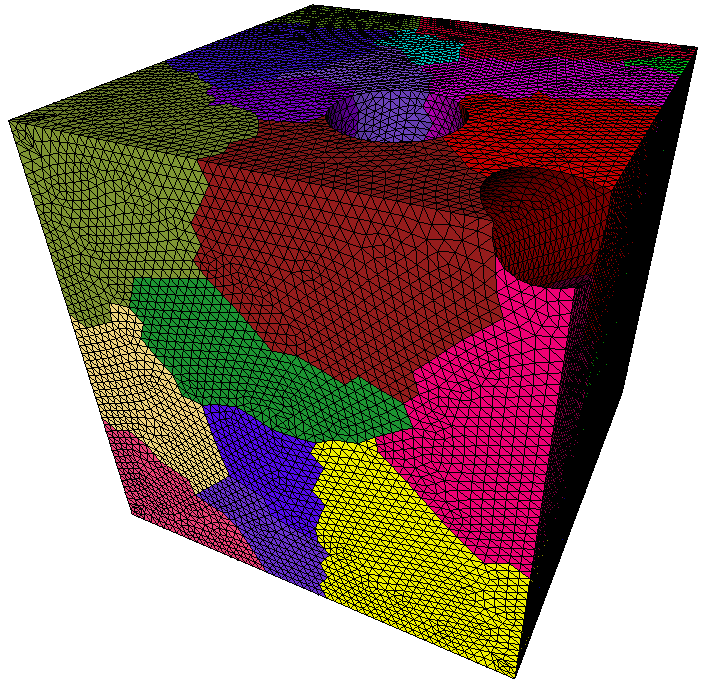
\includegraphics[width=.65\columnwidth]{figures/part_trans} \\
    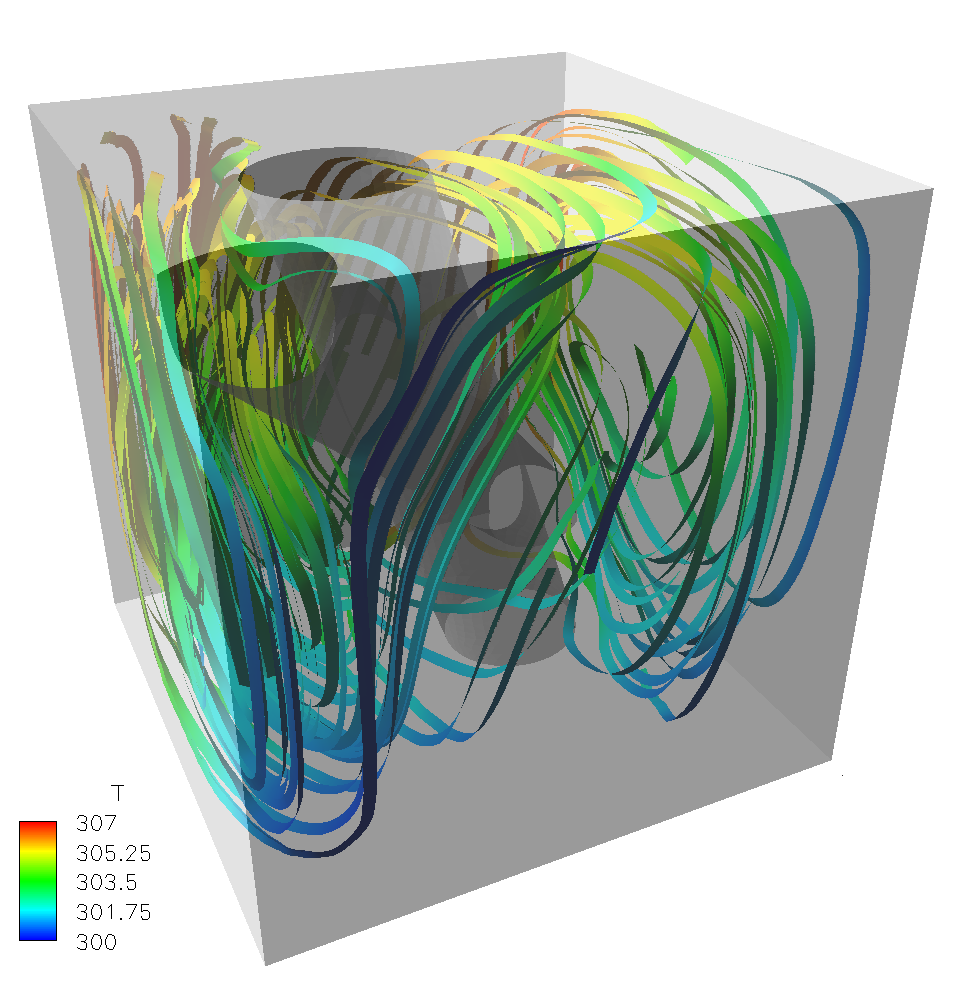
\includegraphics[width=.65\columnwidth]{figures/streamtraces}
    \caption{Buoyancy driven flow in a complex geometry, solved
      in parallel on a workstation cluster.  The upper
      figure shows the METIS partitioning of a tetrahedral mesh
      interior to a cube domain and exterior to two
      cylindrical ``pipes''.  The lower figure depicts stream
      ribbons colored by temperature.  The fluid is naturally convected
      away from the hot wall of the domain and forms a complex circulation
      field around the pipe geometry.\label{fig:rayleigh}}
  \end{center}
\end{figure}

\begin{figure}[hbt]
  \begin{center}
    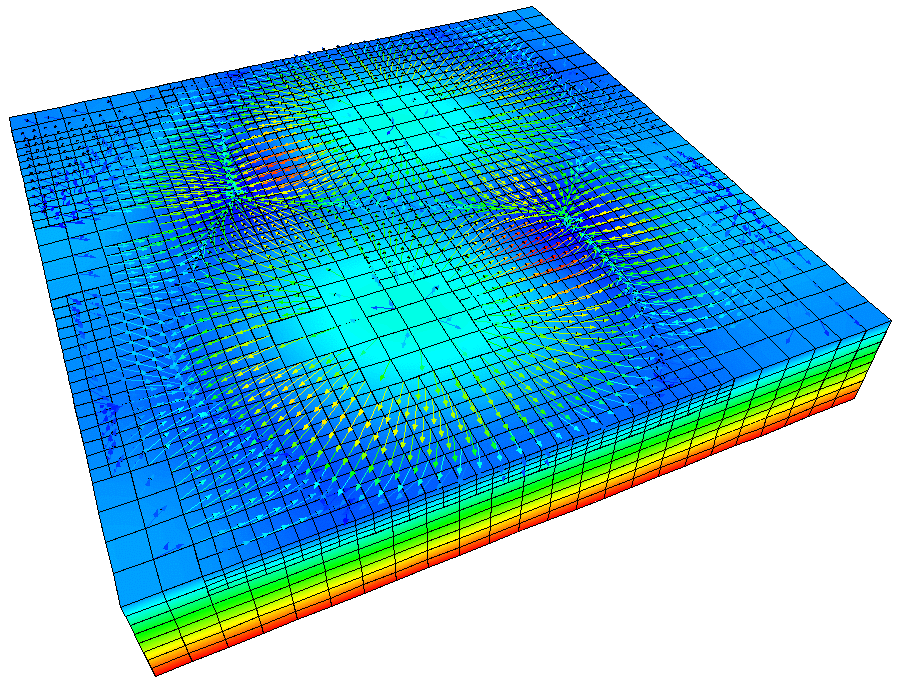
\includegraphics[width=\columnwidth]{figures/rbm_adapt_soln}    
    \caption{Thermocapillary surface-tension
      (Rayleigh-B$\acute{\text{e}}$nard-Marangoni) flow application with
      adaptivity, solved in parallel on a workstation cluster.
      Temperature contours are shown, with warmer
      fluid rising from the bottom of the domain due to buoyancy and
      then spreading when it reaches the surface due to
      thermocapillary effects.  Also shown are surface velocity
      vectors and localized refinement driven by velocity gradients at
      the developing convection cell boundaries.
      \label{fig:rbm}}
  \end{center}
\end{figure}

\begin{figure}[hbt]
  \begin{center}
    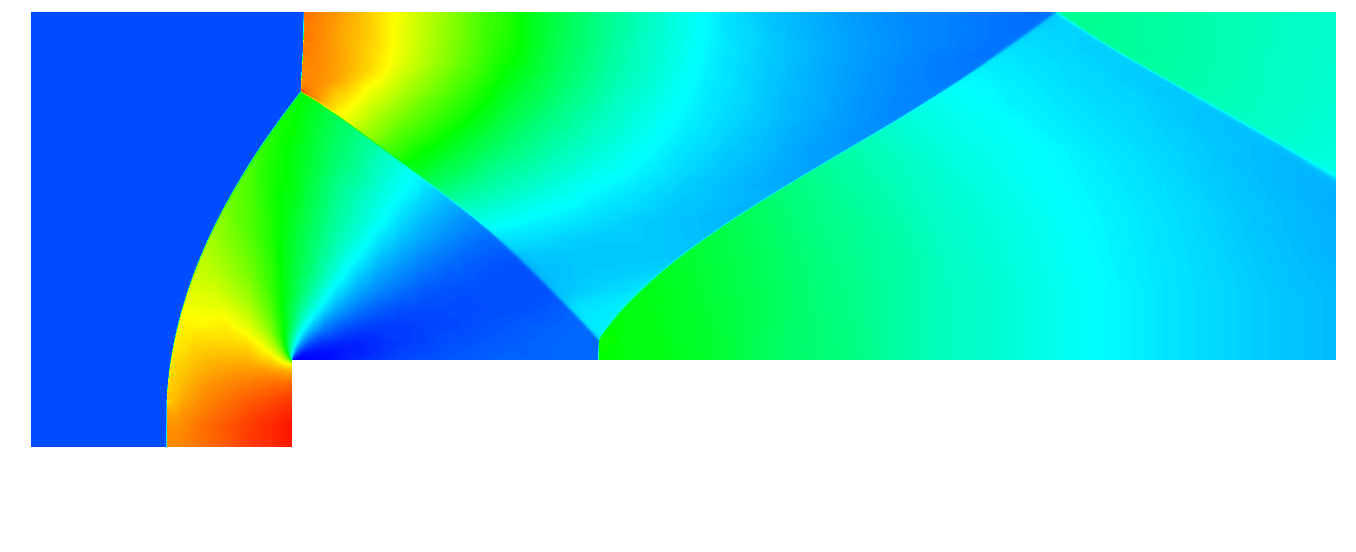
\includegraphics[width=\columnwidth]{figures/wt_m3_p} \\
    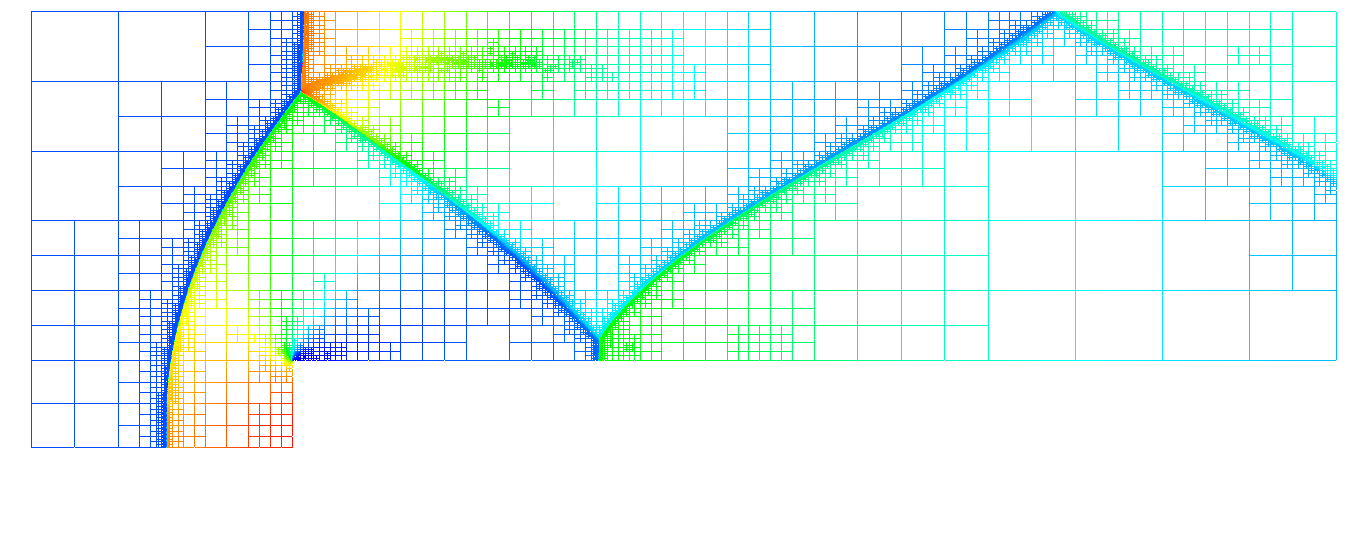
\includegraphics[width=\columnwidth]{figures/wt_m3_p_mesh}
    \caption{Pressure field for Mach~3 inviscid flow over a forward
    facing step.  In this case, the adaptivity is driven by
    inter-element jumps in velocity and tracks normal and oblique
    shock waves in the flow.  The contact surface emanating from the
    Mach stem near top of the domain, a constant pressure structure
    separating regions of supersonic and subsonic flow, is naturally
    tracked by the indicator as well.
    \label{fig:wt_m3}}
  \end{center}
\end{figure}

\begin{figure}[hbt]
  \begin{center}
    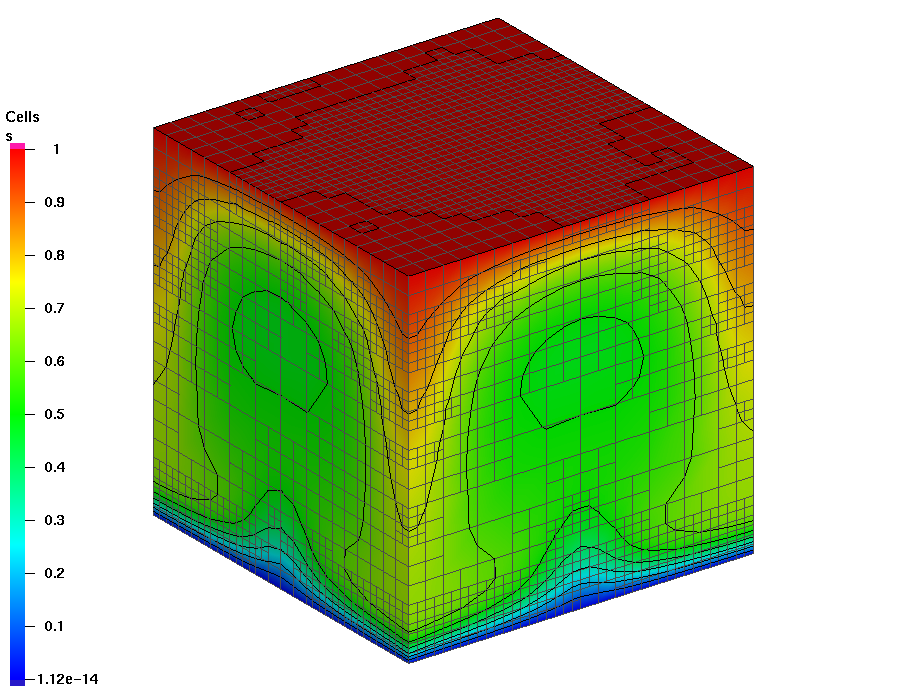
\includegraphics[width=\columnwidth]{figures/dd}    
    \caption{Solute contours in a 3D adaptive simulation of
      double-diffusive convection in a porous medium.  A plume of
      warm, low concentration fluid is convected upward, and a solute
      boundary layer develops near the bottom of the domain.  The adaptivity
      is driven by a physics-independent indicator as discussed in
      Section~\ref{sec:amrc}, which in this case is related to inter-element
      jumps in the solutal flux.
      \label{fig:dd}}
  \end{center}
\end{figure}

\begin{figure}[hbt]
  \begin{center}
    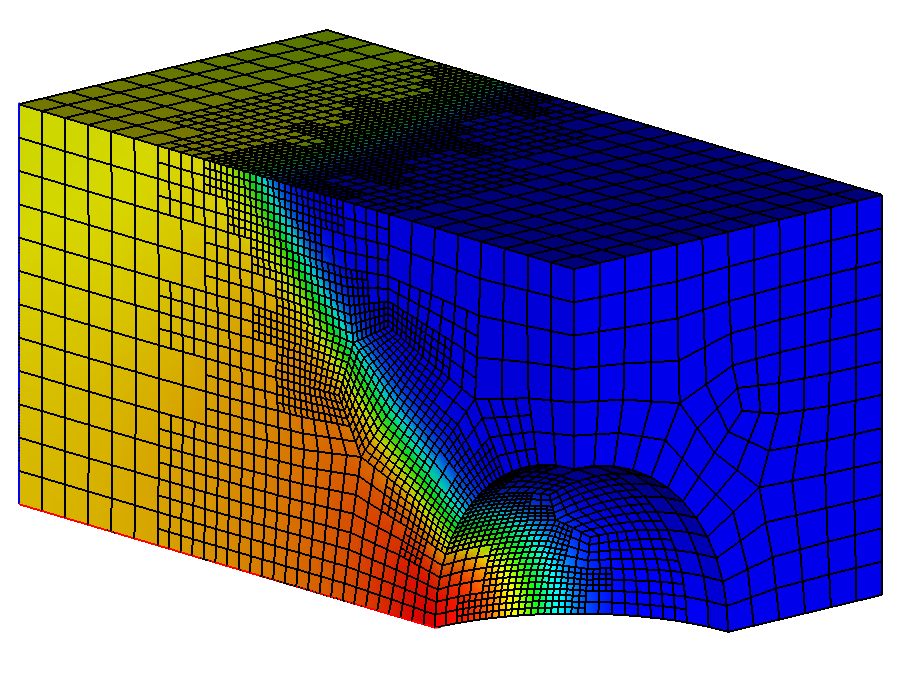
\includegraphics[width=\columnwidth]{figures/tumor_model}    
    \caption{Adaptive 3D solution to the tumor angiogenesis problem
      conducted on 64 processors.  
      This application models an extension of the 2D model considered
      by Valenciano and Chaplain~\cite{VaCh04}.  The tumor,
      represented by the cut-out spherical region, secretes a chemical
      which attracts endothelial cells (represented by the contours)
      and eventually leads to the birth of new blood vessels which feed
      the tumor.  In this simulation, AMR using a physics-independent
      error indicator tracks the advancing front of endothelial cells.
      \label{fig:tumor_model}}
  \end{center}
\end{figure}

Application areas for the wider \libMesh{} community include
electrostatics in thin films of silicon and composite materials,
linear elasticity with Cauchy-Born constitutive models, Stokes flow
with free capillary boundaries, optical imaging, Helmholtz and wave
equations for interior and exterior domains, eigenvalue/modal
analysis, 3D geoelectric solvers with infinite elements for potential
field continuation, magnetic resonance simulation, nonlinear heat
conduction, cavity radiation, thermoelastic problems in solid
mechanics, calcium dynamics in cardiac cells, and Lagrangian particle
tracking.  For additional references in which \libMesh{} was used as
part of the solution methodology,
see~\cite{modelling_error,Tumor,Simedrea_CSCBC,Schindler_2005,carey_bail_2004,PeteS06,DreyD06,BrinM06,lu_2005_biophysical_poster}.

It is important to note that solution algorithms are necessarily
highly problem-dependent. This is underscored by contrasting the
solution algorithms used for compressible flows
(figure~\ref{fig:wt_m3}) and incompressible flows
(figures~\ref{fig:rayleigh} and~\ref{fig:rbm}). The nonlinear problem
arising in implicit algorithms for compressible flows is notoriously
sensitive to the initial guess, hence time stepping to steady-state is
a common technique for solving these problems.  At a given time step
the resulting nonlinear problem is only approximately solved.  For
this application, the run-time is essentially split between matrix
assembly and executing linear solves.  By contrast, steady
incompressible flows result in a nonlinear system which is
considerably less sensitive to initial guess.  These applications may
be solved either steady or via time marching with a small number of
time steps.  In this case, the nonlinear problem is solved to much
higher accuracy.  A typical incompressible flow application may spend
15\% of run-time in matrix assembly with the remaining 85\% spent in
solving the linear system to a high accuracy.

 \libMesh{} provides a wide range of building blocks for steady or
transient, linear or nonlinear, implicit or explicit, static or
dynamic mesh algorithms (and combinations thereof).  As mentioned
previously, many algorithmic details such as linear solver tolerances,
refinement criteria, mesh partitioning quality, etc.\ interplay in
these advanced applications.  It is not appropriate for a
physics-independent library to make these choices, and thus in
\libMesh{} they are controlled by the user. Numerical experiments are
key for finding the optimal solution algorithm for a given
application.
%% %
%% % For two-column wide figures use
%% \begin{figure*}
%% % Use the relevant command for your figure-insertion program
%% % to insert the figure file. See example above.
%% % If not, use
%% \vspace*{5cm}       % Give the correct figure height in cm
%% \caption{Please write your figure caption here}
%% \label{fig:2}       % Give a unique label
%% \end{figure*}
%

%% % For tables use
%% \begin{table}
%% \caption{Please write your table caption here}
%% \label{tab:1}       % Give a unique label
%% % For LaTeX tables use
%% \begin{tabular}{lll}
%% \hline\noalign{\smallskip}
%% first & second & third  \\
%% \noalign{\smallskip}\hline\noalign{\smallskip}
%% number & number & number \\
%% number & number & number \\
%% \noalign{\smallskip}\hline
%% \end{tabular}
%% % Or use
%% \vspace*{5cm}  % with the correct table height
%% \end{table}



%%%%%%%%%%%%%%%%%%%%%%%%%%%%%%%%%%%%%%%%%%%%%%%%%%%%%%%%%%%%%%%%%%%%%%%%%%%%%%
\section{Concluding Remarks and Future Plans\label{sec:conclusion}}
As illustrated in the applications sample, \libMesh{}
provides a powerful capability for efficient and accurate adaptive
finite element solutions of diverse applications in a serial or
parallel environment.  It requires a nominal initial effort by the
applications analyst to encode in \cpp{} a Jacobian and residual
description, and some understanding of the application to select
better tolerances than the default values may provide.  The library
permits AMR/C simulations on different architectures including Linux
clusters and can handle hybrid meshes using a 2-level AMR/C scheme
with hanging nodes.  It has been tested by the \CFDLab{} members for
Galerkin, Petrov-Galerkin, and Discontinuous Galerkin schemes.
Standard $C^0$ and $C^1$ finite elements as well as infinite elements
are supported.

%% A distinguishing feature of the library is its inclusion of
%% so-called infinite elements for acoustics and wave propagation
%% problems.  A small research group from Technische Universit\"{a}t
%% Hamburg-Harburg in Germany is responsible for the creation and
%% maintenance of this code capability.  To our knowledge, \libMesh{}
%% is the only high performance open source finite element library
%% that currently provides these elements.

Some of the issues that we are addressing include recovery and other
physics-independent error indicators.  Future studies may involve
closer linkage to specific application codes, the use of more
sophisticated dual indicators, and the development of error indicators
suited to fully automatic $hp$ adaptivity.  Augmentation by mesh
smoothing and redistribution is also an interesting area, particularly
from the standpoint of adaptivity, since smoothing can be conducted at
the coarsest mesh level.  Combined adaptive
refinement-redist\-ribution-smoothing techniques will likely require
conforming and/or anisotropic refinement strategies, both of which are
areas for future library improvement.  The algorithm for simultaneous
refinement and coarsening is also being improved.  This will involve
studies regarding the selection of tolerances for refinement and
solution steps, and impact the frequency of dynamic repartitioning.

Finally, a fully parallelized implementation of the basic unstructured
mesh data structure is being explored.  The current implementation
duplicates the global mesh on each processor and is clearly a
limitation for scalability and maximum problem size.  Also, mesh class
specializations for Cartesian and block-structured grids are also
being considered.  The mesh data structures have been designed to
allow for specific implementations to handle these special cases.

\section{Acknowledgments}
The student authors of \libMesh{} have been partially supported by a
Department of Energy Computational Science Graduate Fellowship,
Institute for Computational and Engineering Sciences (ICES)
fellowships, N\-A\-SA Graduate Student Research Grant NGT5-139, and
DARPA Grant No. HR\-0011-06-1-0005.

David Knezevic performed the tumor angiogenesis simulation and
implemented support for 1D problems in the library.  Varis Carey
provided a patch recovery error indicator implementation.  Infinite
elements, support for complex-valued systems, and eigenvalue problems
were provided by Daniel Dreyer and Steffen Petersen from Technische
Universit\"{a}t Hamburg-Harburg.  Additionally, we are grateful to the
\dealII{} project for inspiring \libMesh{}, and Wolfgang Bangerth in
particular for many useful discussions.

%
% BibTeX users please use
%\bibliographystyle{spbasic}
%\bibliographystyle{ieeetr}
\bibliographystyle{unsrt_spbasic} % Numbering is in order of appearance
\bibliography{paper}
\end{document}



% LocalWords:  CFDLab multiscale multiphysics AMR reusability MPI Galerkin HPC
% LocalWords:  discretization Petrov posteriori Krylov Superconvergence Sandia
% LocalWords:  equidistributed Fortran operability online FEBase QBase Alegra
% LocalWords:  NumericVector SparseMatrix executables profiler LGPL API doxygen
% LocalWords:  Delaunay triangulator METIS ParMETIS Zoltan subclassing Numer ic
% LocalWords:  Partitioner Eigen LASPack Universidad Politecnica de AutoPtr pre
% LocalWords:  OStringStream reimplement Makefile Itanium OSX preprocessor UCD
% LocalWords:  PETSc subdomains subdomain interprocessor parallelized AVS deas
% LocalWords:  UNV GMSH TetGen Tecplot GMV Los Alamos DofObject vertices lookup
% LocalWords:  indices hexahedra tetrahedra subelements quadtree multigrid PDE
% LocalWords:  supersets ExplicitSystem LinearImplicitSystem EigenSystem nard
% LocalWords:  NonlinearImplicitSystem FrequencySystem NewmarkSystem Marangoni
% LocalWords:  noded hexahedral tri LBB discretizations Clough Tocher Astley sp
% LocalWords:  macroelements Jacobian tradeoffs refactoring implementors sha
% LocalWords:  parallelizable multi CPUs multithreading Bcast Navier SUPG Coli
% LocalWords:  thermocapillary aerothermodynamics angiogenesis advection ers
% LocalWords:  solutal Valenciano endothelial geoelectric thermoelastic Harburg
% LocalWords:  Technische Universit redist ribution NGT Knezevic Varis Dreyer
% LocalWords:  Bangerth
